% Options for packages loaded elsewhere
\PassOptionsToPackage{unicode}{hyperref}
\PassOptionsToPackage{hyphens}{url}
\PassOptionsToPackage{dvipsnames,svgnames,x11names}{xcolor}
%
\documentclass[
  12pt,
]{article}
\usepackage{amsmath,amssymb}
\usepackage{iftex}
\ifPDFTeX
  \usepackage[T1]{fontenc}
  \usepackage[utf8]{inputenc}
  \usepackage{textcomp} % provide euro and other symbols
\else % if luatex or xetex
  \usepackage{unicode-math} % this also loads fontspec
  \defaultfontfeatures{Scale=MatchLowercase}
  \defaultfontfeatures[\rmfamily]{Ligatures=TeX,Scale=1}
\fi
\usepackage{lmodern}
\ifPDFTeX\else
  % xetex/luatex font selection
\fi
% Use upquote if available, for straight quotes in verbatim environments
\IfFileExists{upquote.sty}{\usepackage{upquote}}{}
\IfFileExists{microtype.sty}{% use microtype if available
  \usepackage[]{microtype}
  \UseMicrotypeSet[protrusion]{basicmath} % disable protrusion for tt fonts
}{}
\makeatletter
\@ifundefined{KOMAClassName}{% if non-KOMA class
  \IfFileExists{parskip.sty}{%
    \usepackage{parskip}
  }{% else
    \setlength{\parindent}{0pt}
    \setlength{\parskip}{6pt plus 2pt minus 1pt}}
}{% if KOMA class
  \KOMAoptions{parskip=half}}
\makeatother
\usepackage{xcolor}
\usepackage[margin = 1.2in]{geometry}
\usepackage{color}
\usepackage{fancyvrb}
\newcommand{\VerbBar}{|}
\newcommand{\VERB}{\Verb[commandchars=\\\{\}]}
\DefineVerbatimEnvironment{Highlighting}{Verbatim}{commandchars=\\\{\}}
% Add ',fontsize=\small' for more characters per line
\usepackage{framed}
\definecolor{shadecolor}{RGB}{248,248,248}
\newenvironment{Shaded}{\begin{snugshade}}{\end{snugshade}}
\newcommand{\AlertTok}[1]{\textcolor[rgb]{0.94,0.16,0.16}{#1}}
\newcommand{\AnnotationTok}[1]{\textcolor[rgb]{0.56,0.35,0.01}{\textbf{\textit{#1}}}}
\newcommand{\AttributeTok}[1]{\textcolor[rgb]{0.13,0.29,0.53}{#1}}
\newcommand{\BaseNTok}[1]{\textcolor[rgb]{0.00,0.00,0.81}{#1}}
\newcommand{\BuiltInTok}[1]{#1}
\newcommand{\CharTok}[1]{\textcolor[rgb]{0.31,0.60,0.02}{#1}}
\newcommand{\CommentTok}[1]{\textcolor[rgb]{0.56,0.35,0.01}{\textit{#1}}}
\newcommand{\CommentVarTok}[1]{\textcolor[rgb]{0.56,0.35,0.01}{\textbf{\textit{#1}}}}
\newcommand{\ConstantTok}[1]{\textcolor[rgb]{0.56,0.35,0.01}{#1}}
\newcommand{\ControlFlowTok}[1]{\textcolor[rgb]{0.13,0.29,0.53}{\textbf{#1}}}
\newcommand{\DataTypeTok}[1]{\textcolor[rgb]{0.13,0.29,0.53}{#1}}
\newcommand{\DecValTok}[1]{\textcolor[rgb]{0.00,0.00,0.81}{#1}}
\newcommand{\DocumentationTok}[1]{\textcolor[rgb]{0.56,0.35,0.01}{\textbf{\textit{#1}}}}
\newcommand{\ErrorTok}[1]{\textcolor[rgb]{0.64,0.00,0.00}{\textbf{#1}}}
\newcommand{\ExtensionTok}[1]{#1}
\newcommand{\FloatTok}[1]{\textcolor[rgb]{0.00,0.00,0.81}{#1}}
\newcommand{\FunctionTok}[1]{\textcolor[rgb]{0.13,0.29,0.53}{\textbf{#1}}}
\newcommand{\ImportTok}[1]{#1}
\newcommand{\InformationTok}[1]{\textcolor[rgb]{0.56,0.35,0.01}{\textbf{\textit{#1}}}}
\newcommand{\KeywordTok}[1]{\textcolor[rgb]{0.13,0.29,0.53}{\textbf{#1}}}
\newcommand{\NormalTok}[1]{#1}
\newcommand{\OperatorTok}[1]{\textcolor[rgb]{0.81,0.36,0.00}{\textbf{#1}}}
\newcommand{\OtherTok}[1]{\textcolor[rgb]{0.56,0.35,0.01}{#1}}
\newcommand{\PreprocessorTok}[1]{\textcolor[rgb]{0.56,0.35,0.01}{\textit{#1}}}
\newcommand{\RegionMarkerTok}[1]{#1}
\newcommand{\SpecialCharTok}[1]{\textcolor[rgb]{0.81,0.36,0.00}{\textbf{#1}}}
\newcommand{\SpecialStringTok}[1]{\textcolor[rgb]{0.31,0.60,0.02}{#1}}
\newcommand{\StringTok}[1]{\textcolor[rgb]{0.31,0.60,0.02}{#1}}
\newcommand{\VariableTok}[1]{\textcolor[rgb]{0.00,0.00,0.00}{#1}}
\newcommand{\VerbatimStringTok}[1]{\textcolor[rgb]{0.31,0.60,0.02}{#1}}
\newcommand{\WarningTok}[1]{\textcolor[rgb]{0.56,0.35,0.01}{\textbf{\textit{#1}}}}
\usepackage{graphicx}
\makeatletter
\def\maxwidth{\ifdim\Gin@nat@width>\linewidth\linewidth\else\Gin@nat@width\fi}
\def\maxheight{\ifdim\Gin@nat@height>\textheight\textheight\else\Gin@nat@height\fi}
\makeatother
% Scale images if necessary, so that they will not overflow the page
% margins by default, and it is still possible to overwrite the defaults
% using explicit options in \includegraphics[width, height, ...]{}
\setkeys{Gin}{width=\maxwidth,height=\maxheight,keepaspectratio}
% Set default figure placement to htbp
\makeatletter
\def\fps@figure{htbp}
\makeatother
\setlength{\emergencystretch}{3em} % prevent overfull lines
\providecommand{\tightlist}{%
  \setlength{\itemsep}{0pt}\setlength{\parskip}{0pt}}
\setcounter{secnumdepth}{5}
\newlength{\cslhangindent}
\setlength{\cslhangindent}{1.5em}
\newlength{\csllabelwidth}
\setlength{\csllabelwidth}{3em}
\newlength{\cslentryspacingunit} % times entry-spacing
\setlength{\cslentryspacingunit}{\parskip}
\newenvironment{CSLReferences}[2] % #1 hanging-ident, #2 entry spacing
 {% don't indent paragraphs
  \setlength{\parindent}{0pt}
  % turn on hanging indent if param 1 is 1
  \ifodd #1
  \let\oldpar\par
  \def\par{\hangindent=\cslhangindent\oldpar}
  \fi
  % set entry spacing
  \setlength{\parskip}{#2\cslentryspacingunit}
 }%
 {}
\usepackage{calc}
\newcommand{\CSLBlock}[1]{#1\hfill\break}
\newcommand{\CSLLeftMargin}[1]{\parbox[t]{\csllabelwidth}{#1}}
\newcommand{\CSLRightInline}[1]{\parbox[t]{\linewidth - \csllabelwidth}{#1}\break}
\newcommand{\CSLIndent}[1]{\hspace{\cslhangindent}#1}
\ifLuaTeX
\usepackage[bidi=basic]{babel}
\else
\usepackage[bidi=default]{babel}
\fi
\babelprovide[main,import]{polish}
% get rid of language-specific shorthands (see #6817):
\let\LanguageShortHands\languageshorthands
\def\languageshorthands#1{}
\counterwithin{figure}{section}
\counterwithin{table}{section}
\usepackage[document]{ragged2e}
\usepackage{float}
\floatplacement{figure}{H}
\usepackage[all]{nowidow}
\usepackage{placeins}
\usepackage{fancyhdr}
\usepackage{setspace}
\onehalfspacing
\usepackage{chngcntr}
\usepackage{microtype}
\ifLuaTeX
  \usepackage{selnolig}  % disable illegal ligatures
\fi
\IfFileExists{bookmark.sty}{\usepackage{bookmark}}{\usepackage{hyperref}}
\IfFileExists{xurl.sty}{\usepackage{xurl}}{} % add URL line breaks if available
\urlstyle{same}
\hypersetup{
  pdflang={pl-PL},
  colorlinks=true,
  linkcolor={blue},
  filecolor={Maroon},
  citecolor={Blue},
  urlcolor={blue},
  pdfcreator={LaTeX via pandoc}}

\author{}
\date{\vspace{-2.5em}}

\begin{document}

\def\figurename{Rysunek}

\thispagestyle{empty}

\begin{centering}

\vspace{1 cm}

\includegraphics{Rysunki/Logo/UEW_poziom_RGB_kolor_1.png}

\vspace{1.5 cm}

\LARGE
\bf Projekt zaliczeniowy

\vspace{1.5 cm}

\Large
\textit {Przegląd literatury naukowej z wykorzystaniem narzędzi data science}
\vspace{1 cm}

\large
Studia podyplomowe: Data Science: poziom podstawowy
\vspace{5 cm}

\begin{FlushLeft}
\normalsize
Autor: Grzegorz Kulczycki
\end{FlushLeft}

\vspace{2.5 cm}

\normalsize
Wrocław, 2024

\end{centering}

\newpage
\pagestyle{fancy}

\fancyhead[L,R]{}
\fancyhead[L,R]{}
\renewcommand{\headrulewidth}{0.4pt}
\renewcommand{\footrulewidth}{0pt}

\fancyhead[C]{Streszczenie}
\section*{Streszczenie}
\addcontentsline{toc}{section}{Streszczenie}
\justify

W projekcie przedstawiono możliwości wykorzystana narzędzi data science
do bibliometrycznego przeglądu literatury naukowej. Do analizy
wykorzystano dwie bazy danych \textbf{Google Scholar} oraz
\textbf{Semantic Scholar}. Wykonane analizy potwierdzają dużą
skuteczność i użyteczność zastosowanych narzędzi data science. Narzędzia
te w istotny sposób przyspieszają i zwiększają efektywność
przeprowadzenia przeglądu literatury naukowej w porównaniu z
tradycyjnymi metodami ich wykonywania.

\newpage
\fancyhead[C]{Podziękowania}
\section*{Podziękowania}

Składam serdeczne podziękowania dla \textbf{mgr Agnieszki Rosa} za
zaangażowanie i merytoryczną pomoc.

\newpage
\fancyhead[C]{Spis treści}
\setcounter{tocdepth}{2}
\tableofcontents
\addcontentsline{toc}{section}{Spis treści}

\newpage

\newpage
\fancyhead[C]{Wstęp i określenie celu badań}

\hypertarget{wstux119p-i-cel-badaux144}{%
\section{\texorpdfstring{Wstęp i cel
badań\label{label1}}{Wstęp i cel badań}}\label{wstux119p-i-cel-badaux144}}

Praca naukowa to określony rodzaj formy pracy twórczej związany z
obiektywnym poznaniem zjawisk, rzeczy oraz różnego rodzaju relacji
pomiędzy nimi. Wyniki prac naukowych przedstawia się w rożnych formach
(książki, raporty,czy sprawozdania) spośród których, najbardziej
popularną metodą jest pisanie artykułów (publikacji) naukowych.

Publikację naukową można zdefiniować w różny sposób w zależności od celu
w jakim została stworzona. Najogólniej publikacją naukową określa się
doniesienie o uzyskanych wynikach badań lub opis istniejącego stanu
wiedzy z określonego obszaru nauki. Artykuły naukowe zamieszczane są w
czasopismach, które publikują je w formie papierowej lub najczęściej
elektronicznej przez wydawnictwa naukowe. Ocena wpływu danych czasopism
odbywa się poprzez analizę bibliometryczną cytowań, gdzie liczba cytowań
artykułów w czasopiśmie stanowi miarę popularności i wpływu czasopisma.
Większość wydawnictw publikujących prace naukowe wykorzystuje własne
strony internetowe do przyjmowania, recenzowania oraz udostępniania
publikowanych prac w trybie on-line.

Naukowcy także podlegają ewaluacji miedzy innymi poprzez systematyczną
ocenę ich dorobku naukowego. Dorobek ten wyceniany jest miedzy innymi w
oparciu o opublikowane artykuły naukowe w czasopismach oraz ilość
cytowań, jakie ten artykuł otrzymał. Ilość i jakość opublikowanych prac
naukowych jest istotna dla pracowników jak i dla instytucji naukowych w
której są zatrudnieni, ponieważ zarówno te podmioty jak również
pracownicy w nich zatrudnieni podlegają okresowej ocenie. Ewaluację
przeprowadza się za okres 4 lat poprzedzających rok jej przeprowadzenia,
z uwzględnieniem osiągnięć naukowych pracowników
(\protect\hyperlink{ref-dz.u.2019}{Dz. U., 2019}). W związku z powyższym
obserwuje się ścisłe wzajemne relacje pomiędzy naukowcami a
wydawnictwami czasopism. Przyczynia się to do powstania dużej ilości
artykułów naukowych, które są indeksowane w tematycznych bazach danych.

\textbf{Cel badań:} znaczący przyrost ilości artykułów w danych
dyscyplinach naukowych nasilają problemy z ich przeglądem i oceną.
Wykonywanie takich przeglądów standardowymi ``ręcznymi'' metodami jest
coraz bardziej czasochłonne i mało efektywne. Celem badan było wykonanie
przeglądu oraz meta-analizy danych literatury naukowej metodami opartymi
o data science, które umożliwiłyby ten etap pracy naukowej znacznie
przyspieszyć i zwiększyć jego efektywność.

\FloatBarrier
\newpage
\fancyhead[C]{Opis problemu badań}

\hypertarget{opis-problemu-badaux144}{%
\section{\texorpdfstring{Opis problemu
badań\label{label1}}{Opis problemu badań}}\label{opis-problemu-badaux144}}

\textbf{Organizacja i etapy badań naukowych}

Podczas prowadzenia badań naukowych wyróżnia się szereg etapów, które
stanowią określoną logiczną procedurę badawczą. Etapy te należny
traktować jako elastyczne elementy postępowania badawczego, jednak układ
ich powinien być zawsze ścisły i racjonalny
\ref{etapy_badan}(modyfikacja własna za
(\protect\hyperlink{ref-apanowicz2005}{Apanowicz, 2005})).

\begin{figure}
\centering
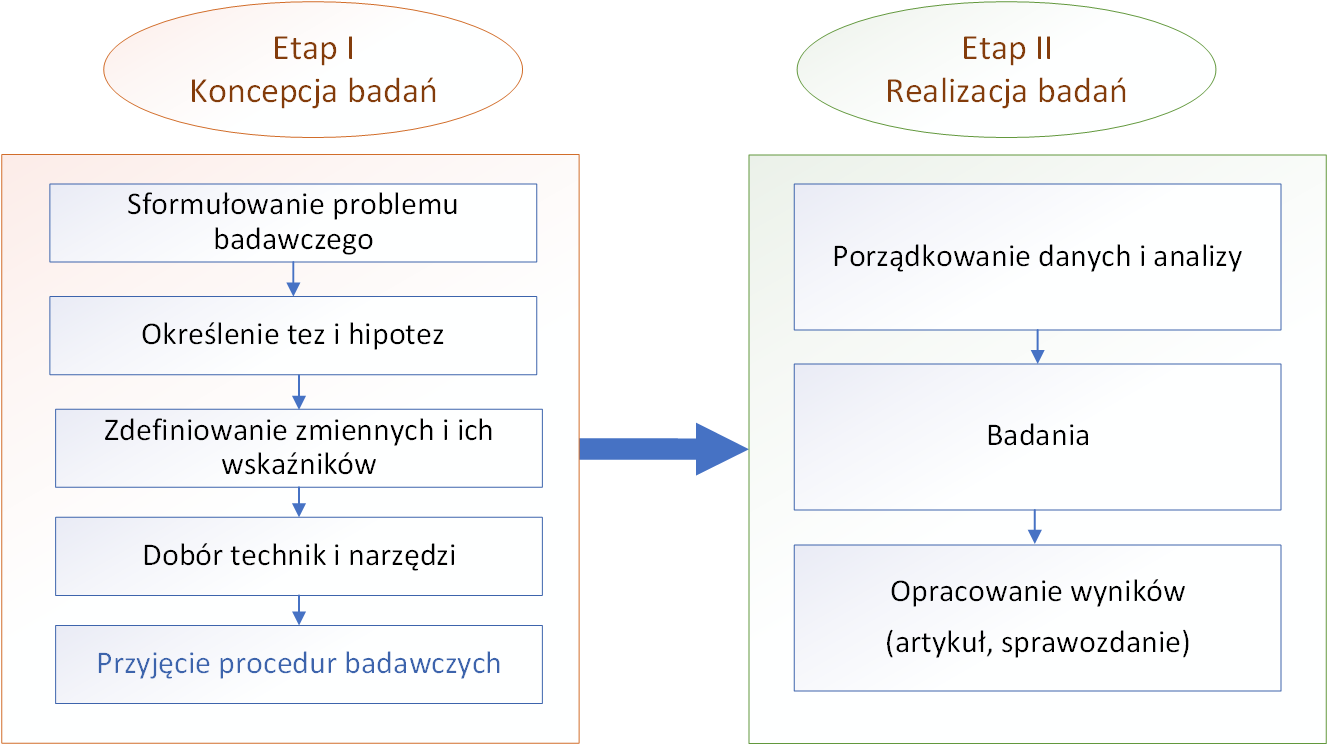
\includegraphics[width=1\textwidth,height=\textheight]{Rysunki/etapy_pracy_badawczej.png}
\caption{Etapy i czynności badań naukowych \label{etapy_badan}}
\end{figure}

Efektem udokumentowania przeprowadzonych badań najczęściej jest
napisanie artykułu naukowego. Uniwersalny schemat często wykorzystywany
podczas realizacji publikacji naukowej przedstawiono na rysunku
\ref{struktura_pub}.

\begin{figure}
\centering
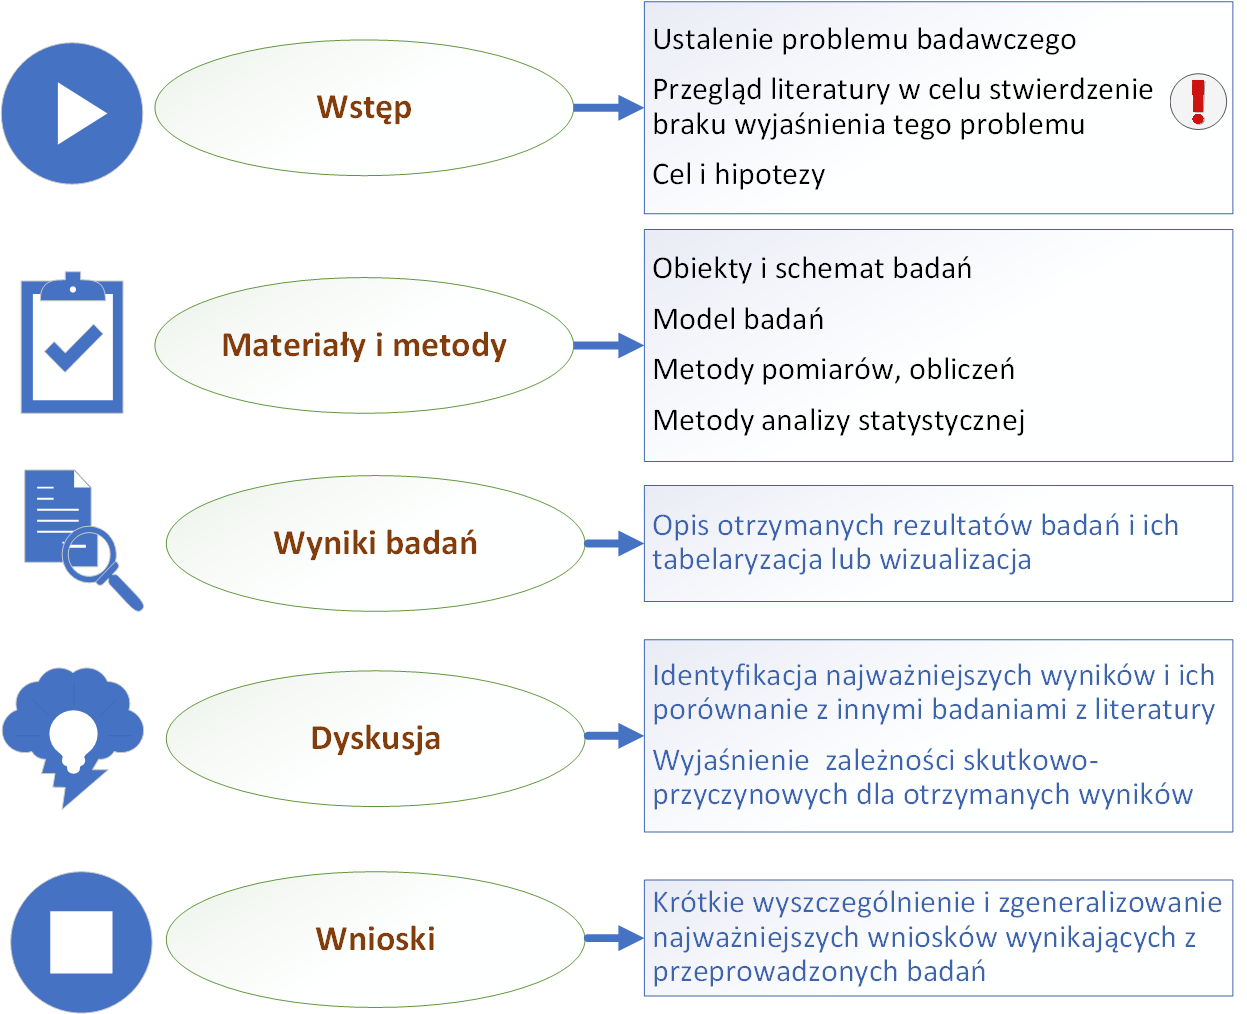
\includegraphics[width=1\textwidth,height=\textheight]{Rysunki/uklad_pracy_badawczej.png}
\caption{Uniwersalna struktuta publikacji naukowej
\label{struktura_pub}}
\end{figure}

Po ustaleniu problemu badawczego i tematu pracy, rozpoczyna się zwykle
etap pracy związany z poszukiwaniem literatury przedmiotu. Celem tego
etapu pracy jest stwierdzenie stanu wiedzy przeszłej i aktualnej
związanej z podjętym tematem badań, określenie brakujących luk i
możliwości ich wypełnienia oraz zasadności poszerzenia wiedzy z danego
obszaru badań (\protect\hyperlink{ref-cooper1986}{Cooper, 1986}) .

Przegląd literatury dotyczy najczęściej publikacji naukowych, które w
obowiązującym obecnie prawie (\protect\hyperlink{ref-dz.u.2019}{Dz. U.,
2019}) w rozumieniu ewaluacji (\protect\hyperlink{ref-pbn2020}{PBN,
2020}) określane są jako: - artykuł naukowy, - monografię naukową, -
rozdział w monografii naukowej.

Słownik Polskiej Bibliografii Naukowej
(\protect\hyperlink{ref-pbn2020}{PBN, 2020}) podaje następujące
definicje publikacji naukowych:

\begin{enumerate}
\def\labelenumi{\arabic{enumi}.}
\tightlist
\item
  Artykuł naukowy jest to recenzowany artykuł opublikowany w czasopiśmie
  naukowym albo w recenzowanych materiałach z międzynarodowych
  konferencji naukowych:
\end{enumerate}

\begin{itemize}
\tightlist
\item
  przedstawiający określone zagadnienie naukowe w sposób oryginalny i
  twórczy, problemowy albo przekrojowy;
\item
  opatrzony przypisami, bibliografią lub innym właściwym dla danej
  dyscypliny naukowej aparatem naukowym.
\end{itemize}

Artykułem naukowym jest również artykuł recenzyjny opublikowany w
czasopiśmie naukowym zamieszczonym w wykazie czasopism.

Artykułem naukowym nie jest: edytorial, abstrakt, rozszerzony abstrakt,
list, errata oraz nota redakcyjna.

\begin{enumerate}
\def\labelenumi{\arabic{enumi}.}
\setcounter{enumi}{1}
\tightlist
\item
  Monografia naukowa jest to recenzowana publikacja książkowa:
\end{enumerate}

\begin{itemize}
\tightlist
\item
  przedstawiająca określone zagadnienie naukowe w sposób oryginalny i
  twórczy;
\item
  opatrzona przypisami, bibliografią lub innym właściwym dla danej
  dyscypliny naukowej aparatem naukowym.
\end{itemize}

Monografią naukową jest również:

\begin{itemize}
\tightlist
\item
  recenzowany i opatrzony przypisami, bibliografią lub innym właściwym
  dla danej dyscypliny naukowej aparatem naukowym przekład na język
  polski dzieła istotnego dla nauki lub kultury albo na inny język
  nowożytny dzieła istotnego dla nauki lub kultury, wydanego w języku
  polskim;
\item
  edycja naukowa tekstów źródłowych.
\end{itemize}

Oceny poziomu naukowego prowadzonej działalności naukowej w zakresie
badań naukowych i prac rozwojowych dokonuje się z uwzględnieniem
następujących rodzajów osiągnięć naukowych
(\protect\hyperlink{ref-dz.u.2019}{Dz. U., 2019}):

\begin{enumerate}
\def\labelenumi{\arabic{enumi}.}
\item
  artykułów naukowych opublikowanych w czasopismach naukowych i w
  recenzowanych materiałach z międzynarodowych konferencji naukowych,
  zamieszczonych w wykazie tych czasopism i materiałów sporządzonym
  zgodnie z przepisami wydanymi na podstawie art. 267 ust. 2 pkt 2
  ustawy, zwanym dalej „wykazem czasopism'';
\item
  artykułów naukowych opublikowanych w czasopismach naukowych
  niezamieszczonych w wykazie czasopism;
\item
  monografii naukowych wydanych przez wydawnictwa zamieszczone w wykazie
  tych wydawnictw sporządzonym zgodnie z przepisami wydanymi na
  podstawie art. 267 ust. 2 pkt 2 ustawy, zwanym dalej „wykazem
  wydawnictw'';
\item
  monografii naukowych wydanych przez wydawnictwa niezamieszczone w
  wykazie wydawnictw, redakcji naukowych takich monografii i autorstwa
  rozdziałów w takich monografiach;
\item
  przyznanych patentów na wynalazki, praw ochronnych na wzory użytkowe i
  wyłącznych praw hodowców do odmian roślin.
\end{enumerate}

Proces publikowania wyników badań obecnie ulega ciągłej modyfikacji i
przyspieszeniu związanym z coraz większym dostępem do Internetu oraz
szybszemu procesowi przyjmowania i recenzji publikacji poprzez strony
własne Wydawnictw.

Szacuje się, że od 1996 roku opublikowano co najmniej 64 miliony
artykułów naukowych, a tempo wzrostu liczby nowo opublikowanych
artykułów \ref{pub_rocznie} ciągle ma tendencje wzrostową
(\protect\hyperlink{ref-curcic2023}{Curcic, 2023}).

\begin{figure}
\centering
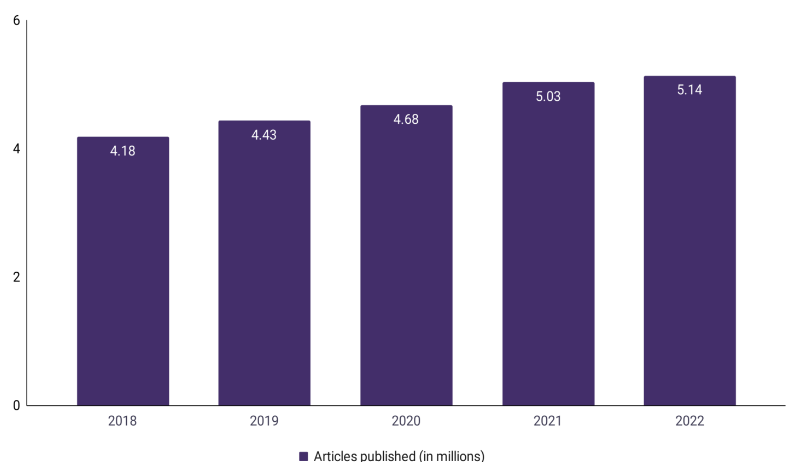
\includegraphics[width=1\textwidth,height=\textheight]{Rysunki/publikacje_rocznie.png}
\caption{Ilość publikowanych artykułów rocznie na świecie
\label{pub_rocznie}}
\end{figure}

Z raportu \href{https://ncses.nsf.gov/indicators}{S\&E - Science and
Engineering Indicators} wynika, że roczny przyrost ilości publikacji na
świecie artykułów naukowo-technicznych wyniósł 4\% w latach 2010-2020
(\protect\hyperlink{ref-curcic2023}{Curcic, 2023}). Na rysunku
\ref{Ilosc_publikacji} zestawiono ilość artykułów naukowo-technicznych
opublikowanych ze wszystkich obszarów nauki na świecie oraz w 15
największych krajach w latach 2010 i 2020.

\begin{figure}
\centering
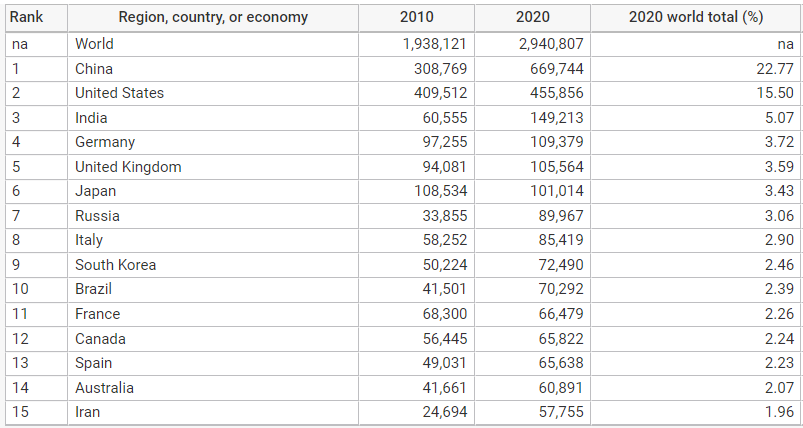
\includegraphics[width=1\textwidth,height=\textheight]{Rysunki/ilosc_opublikowanych_artykulow.png}
\caption{Ilość opublikowanych artykułów naukowo-technicznych
\label{Ilosc_publikacji}}
\end{figure}

Graficzny obraz przyrostu publikowanych artykułów naukowo-technicznych
od roku 1996 przedstawiono na rysunku \ref{grafika_pub_nauk_tech}.
Uwidacznia się na nim wyraźne ogólna tendencja przyrostu publikacji na
świecie, a z pośród analizowanych krajów szczególnie jest to widoczne w
Chinach.

\begin{figure}
\centering
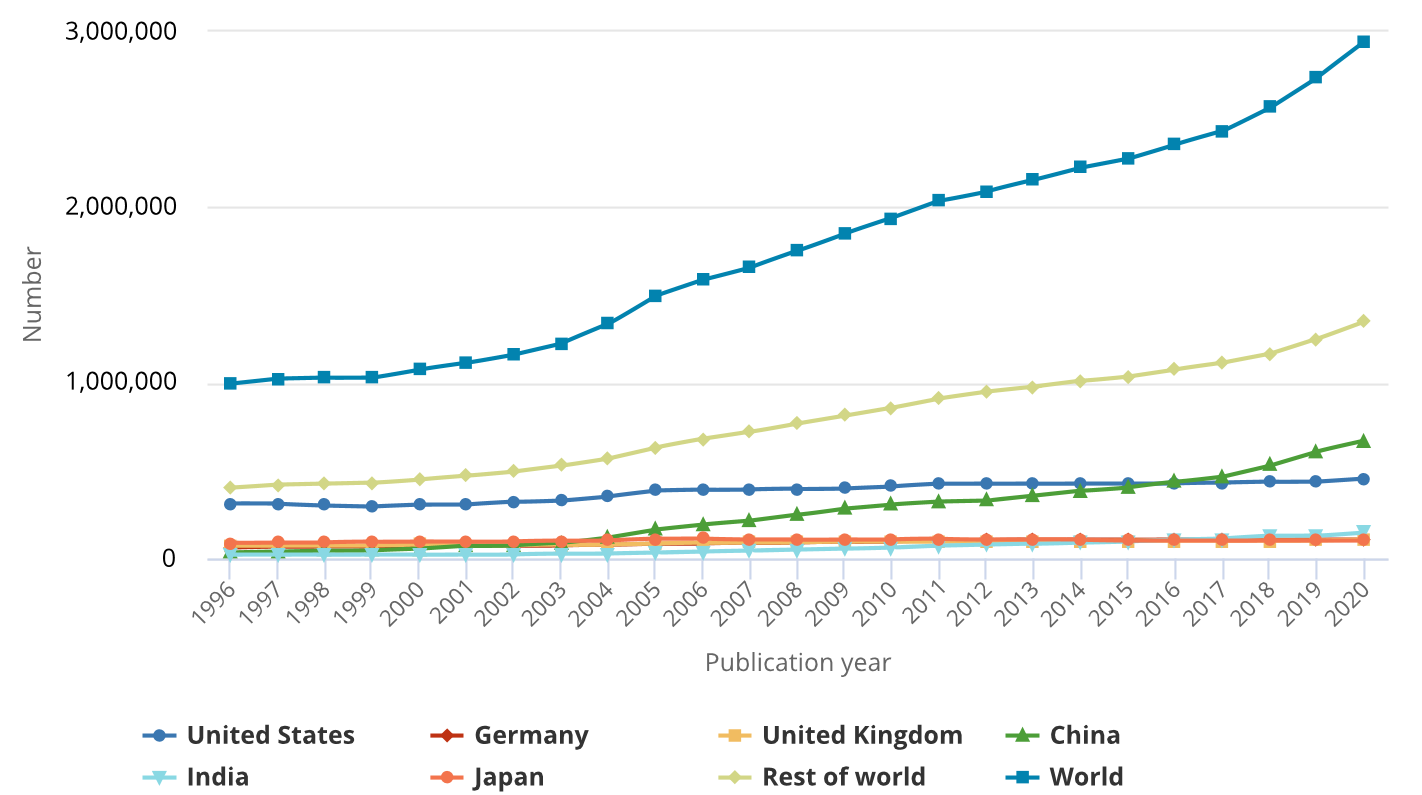
\includegraphics[width=1\textwidth,height=\textheight]{Rysunki/ilosc_pub_graf.png}
\caption{Trendy w ilosci publikowanych artykułów naukowo-technicznych
\label{grafika_pub_nauk_tech}}
\end{figure}

Ilość publikowanych artykułów na świecie koreluje dodatnio ze
wzrastająca ilością czasopism akademickich. W 2020 roku odnotowano 46,7
tys. czasopism \ref{liczba_czasopism}, a ciągu ostatnich 10 lat liczba
ich wzrosła o 29\% (\protect\hyperlink{ref-curcic2023}{Curcic, 2023}).

\begin{figure}
\centering
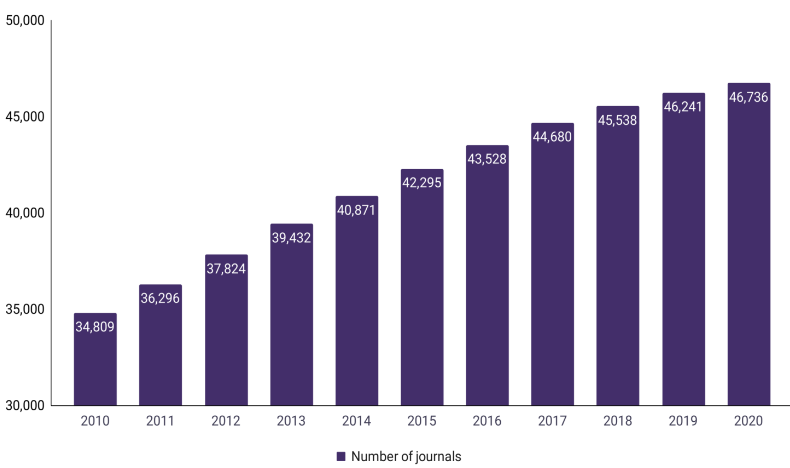
\includegraphics[width=1\textwidth,height=\textheight]{Rysunki/liczba_czasopism.png}
\caption{Ilość czasopism akademickich na świaecie
\label{liczba_czasopism}}
\end{figure}

O wymiarze publikowanych prac naukowych na świecie z zakresu nauk
fizycznych, chemicznych oraz nauk o życiu i środowisku można się
dowiedzieć ze strony \href{https://natureindex.com}{natureindex.com}. Na
podstawie danych (od 1 czerwca 2021 do 31 maja 2022) z tej strony na
rysunku \ref{pub_swiat} wyszczególniono kraje o największej ilości
publikacji. Dane te uwidaczniają, że niekwestionowanymi liderami w tych
obszarach badań są USA oraz Chiny.

\begin{figure}
\centering

\includegraphics{Rysunki/figures/unnamed-chunk-19-1.pdf}
\caption{Kraje o największej ilości publikacji z analizowanego obszarów
badań. \label{pub_swiat}}
\end{figure}

Ilość prac naukowych z tych obszarów badawczych w Europie przedstawiono
na rysunku \ref{pub_europa}, gdzie uwidacznia się, że na kontynencie
europejskim liderami są Wielka Brytania i Niemcy.

\begin{figure}
\centering

\includegraphics{Rysunki/figures/unnamed-chunk-20-1.pdf}
\caption{Ilość publikacji w Europie z analizowanego obszaru badań.
\label{pub_europa}}
\end{figure}

W Polsce opublikowano w tym okresie z tego obszaru badań 906 artykułów
naukowych z pośród których 296 były napisane ze współautorami z innych
krajów. Udział publikacji w poszczególnych obszarach badań przedstawiono
na rysunku \ref{polska_subject}.

\begin{figure}
\centering
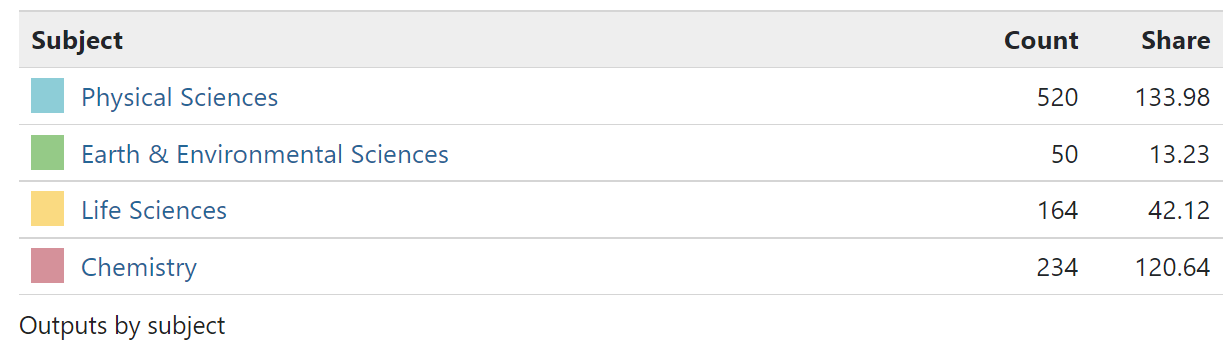
\includegraphics[width=1\textwidth,height=\textheight]{Rysunki/polska_subject.png}
\caption{Ilość publikacji w zależności od obszaru badań.
\label{polska_subject}}
\end{figure}

W latach 2017--2021 opublikowano w Polsce około 619 tys. prac naukowych,
z których większość (67\%) stanowiły artykuły, 29\% -- rozdziały w
monografiach, a pozostałe 4\% -- monografie naukowe
(\protect\hyperlink{ref-pwn2023}{PWN, 2023}).

Tak znaczący przyrost ilości artykułów naukowych nasilają problemy z ich
przeglądem i oceną, która ma na celu znalezienie pytań bez odpowiedzi
lub nierozwiązanych problem w danej dziedzinie.

W pracy naukowej wykonywane są rożnego rodzaju przeglądy literatury w
zależności od celu ich wykonania
(\protect\hyperlink{ref-chigbu2023}{Chigbu i in., 2023}). Zestawienie
rodzajów przeglądów literatury przedstawiono na rysunku
\ref{rodzaje_przeglondow}.

\begin{figure}
\centering
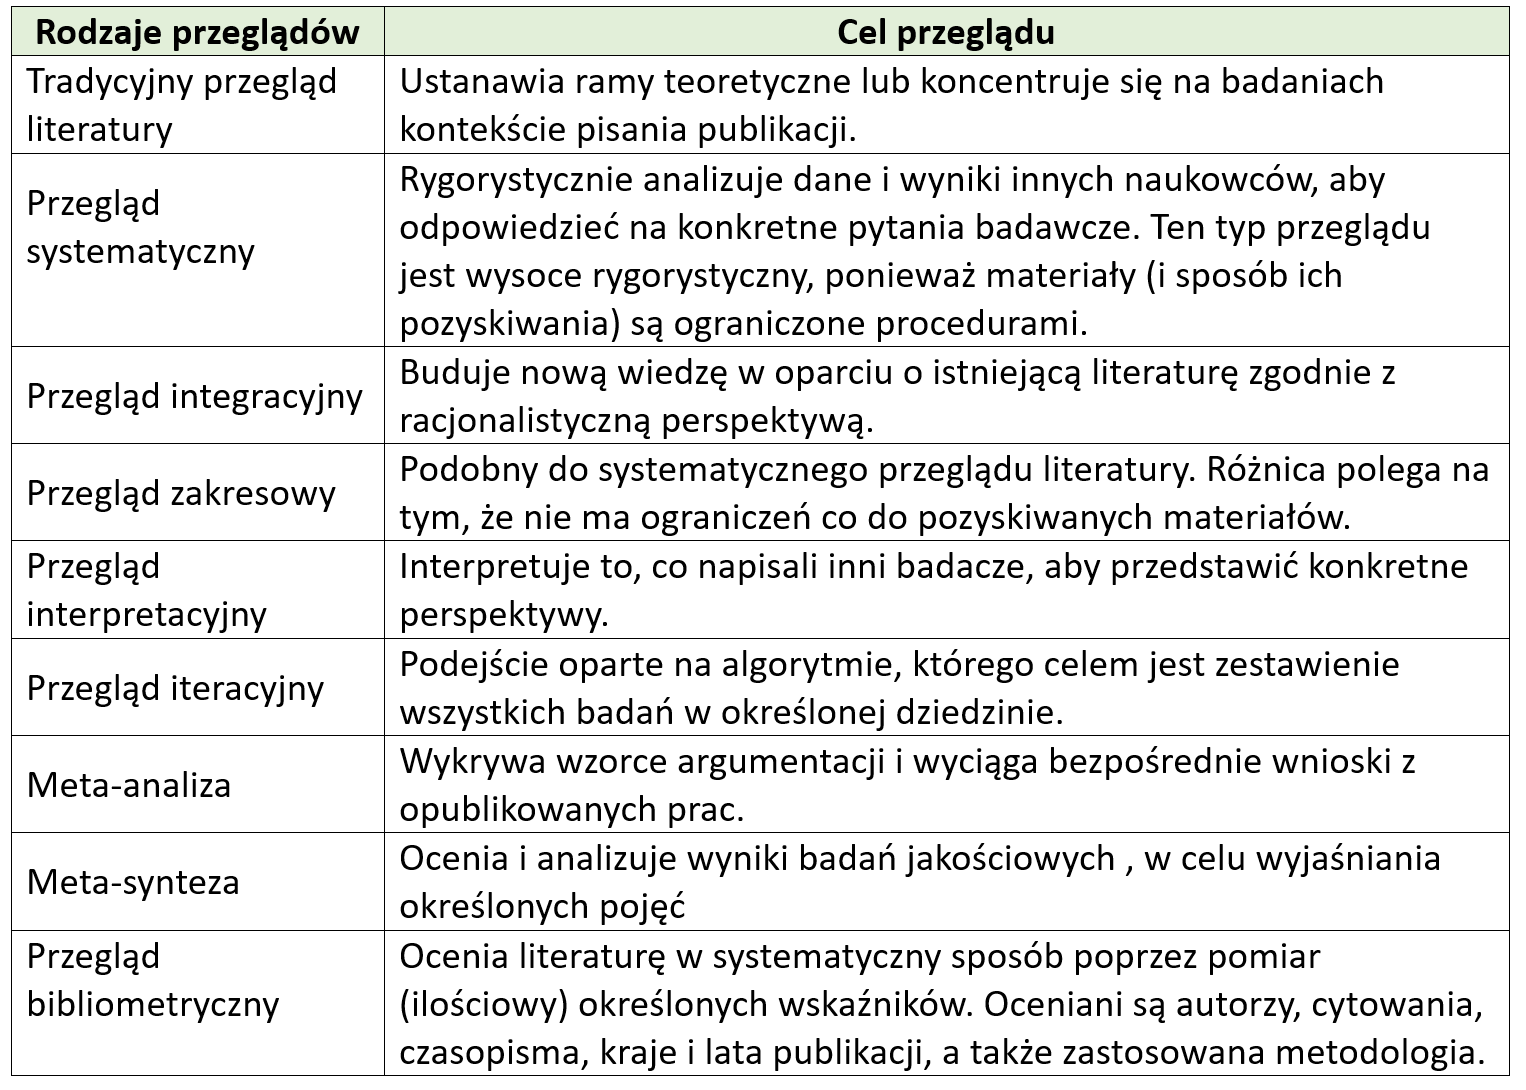
\includegraphics[width=1\textwidth,height=\textheight]{Rysunki/rodzaje_przeglondow.png}
\caption{Rodzaje przegladów literatury\label{rodzaje_przeglondow}}
\end{figure}

\textbf{Bazy danych indeksujące publikacje naukowe}

Odpowiedzią na te wyzwania jest powstanie baz danych indeksujące
istniejące zasoby prac naukowych oraz ich twórców. Wprowadzono w nich
rożne wskaźniki oceniające siłę oddziaływania danej publikacji
(cytowania) oraz oceniające także naukowców (np. wskaźnik Hirscha
h-index).

Obecnie na świecie istnieje znaczna liczba baz danych bibliograficznych.
Szacuje się jednak, że istnieje tysiące bibliograficznych baz danych
dostępnych na całym świecie, obejmujących różne obszary tematyczne,
takie jak medycyna, nauki ścisłe, nauki humanistyczne, nauki społeczne
itp. Nie jest możliwe zestawienia kompletnej listy takich baz, ponieważ
nowe są stale tworzone, podczas gdy inne mogą stać się przestarzałe lub
połączone w większe bazy danych.

Z zestawieniem wybranych i polecanych akademickich baz danych i
wyszukiwarek zapoznać się można na stronie
\href{https://en.wikipedia.org/wiki/List_of_academic_databases_and_search_engines}{Wikipedii}.
Z tego zestawienia subiektywnie wybrano i schrakteryzowano poniżej kilka
baz danych.

Pracownicy nauki korzystają najczęściej z baz danych, takich jak Google
Scholar, Semantic Scholar, Lens, Scopus, Web of Science i ResearchGate w
celu uzyskania dostępu i ocenienia literatury naukowej. Pomiędzy tymi
bazami zauważa się pewne podobieństwa istnieją jednak również istotne
różnice pod względem ich zasięgu, zakresu, możliwości wyszukiwania i
wskaźników cytowań.

\textbf{Charakterystyka wybranych baz indeksujących}

\begin{itemize}
\tightlist
\item
  \href{scholar.google.com}{Google Scholar} najpopularniejsze narzędzie
  ze względu na to, że jest szybkie, bezpłatne i wszechstronne. Usługę
  tą rozpoczęto w listopadzie 2004 r. Kataloguje piśmiennictwo
  akademickie z różnych dziedzin i źródeł, takich jak książki, prace
  dyplomowe, artykuły z czasopism, materiały konferencyjne i preprinty
  (rys. \ref{gogle_scholar}). Obejmuje ona szeroki zakres publikacji, w
  tym takie, które mogą nie być indeksowane przez inne bazy danych.
\end{itemize}

\begin{figure}
\centering

\includegraphics[width=1\textwidth,height=\textheight]{Rysunki/google_scholar.png}
\caption{Google Scholar \label{gogle_scholar}}
\end{figure}

\begin{itemize}
\tightlist
\item
  \href{semanticscholar.org}{Semantic Scholar} baza oparta na metodach
  sztucznej inteligencji, która nadaje priorytet informatyce i badaniom
  biomedycznym (rys. \ref{semantic_scholar}). Indeksuje i kategoryzuje
  artykuły na podstawie ich treści, cytowań i autorów oraz oferuje
  czytelnikom spersonalizowane rekomendacje na podstawie ich historii
  wyszukiwania. Semantic Scholar1 (S2), został uruchomiony w 2015 r.
  przez \href{allenai.org}{Allen Institute for Artificial Intelligence2}
  (AI2), aby pomóc naukowcom w walce z przeciążeniem informacyjnym oraz
  skuteczniejszym odkrywaniu i rozumieniu najistotniejszej literatury
  naukowej.
\end{itemize}

\begin{figure}
\centering
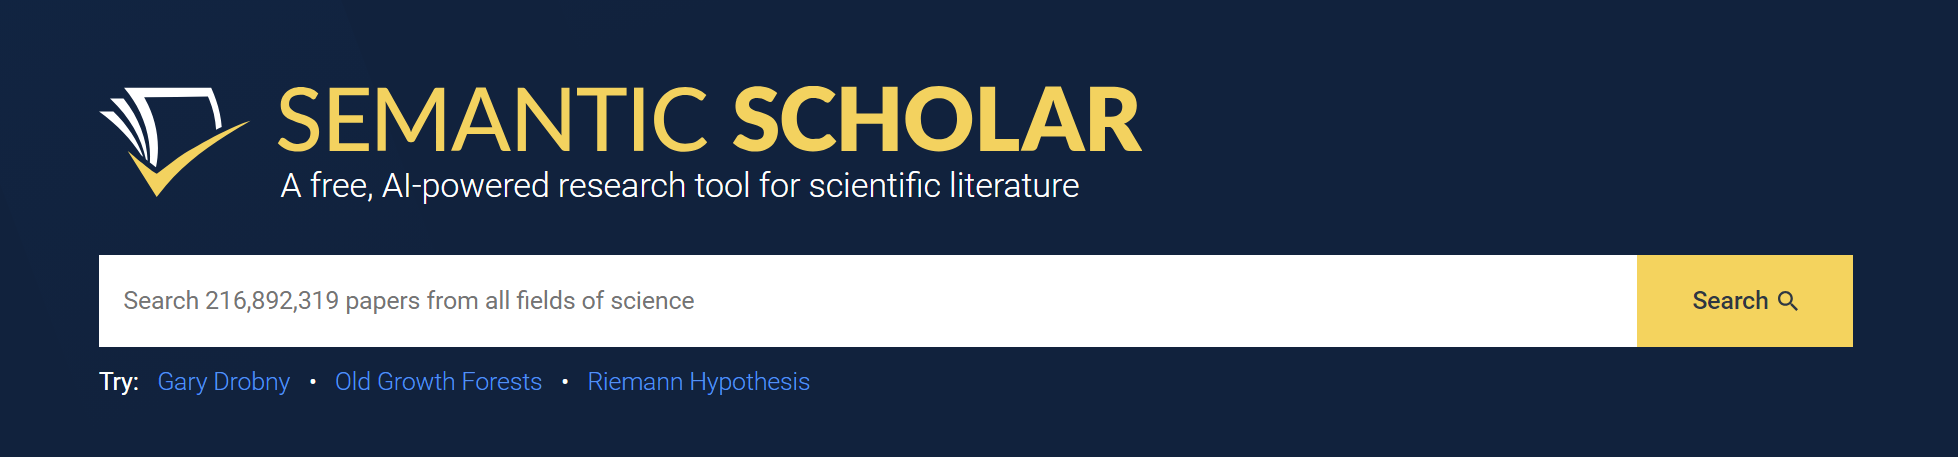
\includegraphics[width=1\textwidth,height=\textheight]{Rysunki/semantic_scholar.png}
\caption{Platforma Semantic Scholar \label{semantic_scholar}}
\end{figure}

Celem Otwartej Platformy Danych Semantic Scholar jest zbudowanie i
rozpowszechnianie Akademickiego Grafu Semantic Scholar lub S2AG
(wymawiane jako ``stag''). S2AG to ujednoznaczniony, wysokiej jakości
bibliograficzny graf wiedzy. Węzły S2AG reprezentują artykuły, autorów,
miejsca i instytucje akademickie. Krawędzie reprezentują artykuły
napisane przez autora, artykuły cytowane przez inny artykuł, artykuły
opublikowane w miejscu i autorów powiązanych z instytucją. S2AG jest
tworzony poprzez wprowadzanie różnych źródeł danych do naszych danych i
jest dystrybuowany za pośrednictwem różnych publicznie dostępnych
interfejsów API i zbiorów danych, jak pokazano na rysunku
\ref{graf_semantic_scholar} (\protect\hyperlink{ref-kinney2023}{Kinney i
in., 2023}).

\begin{figure}
\centering
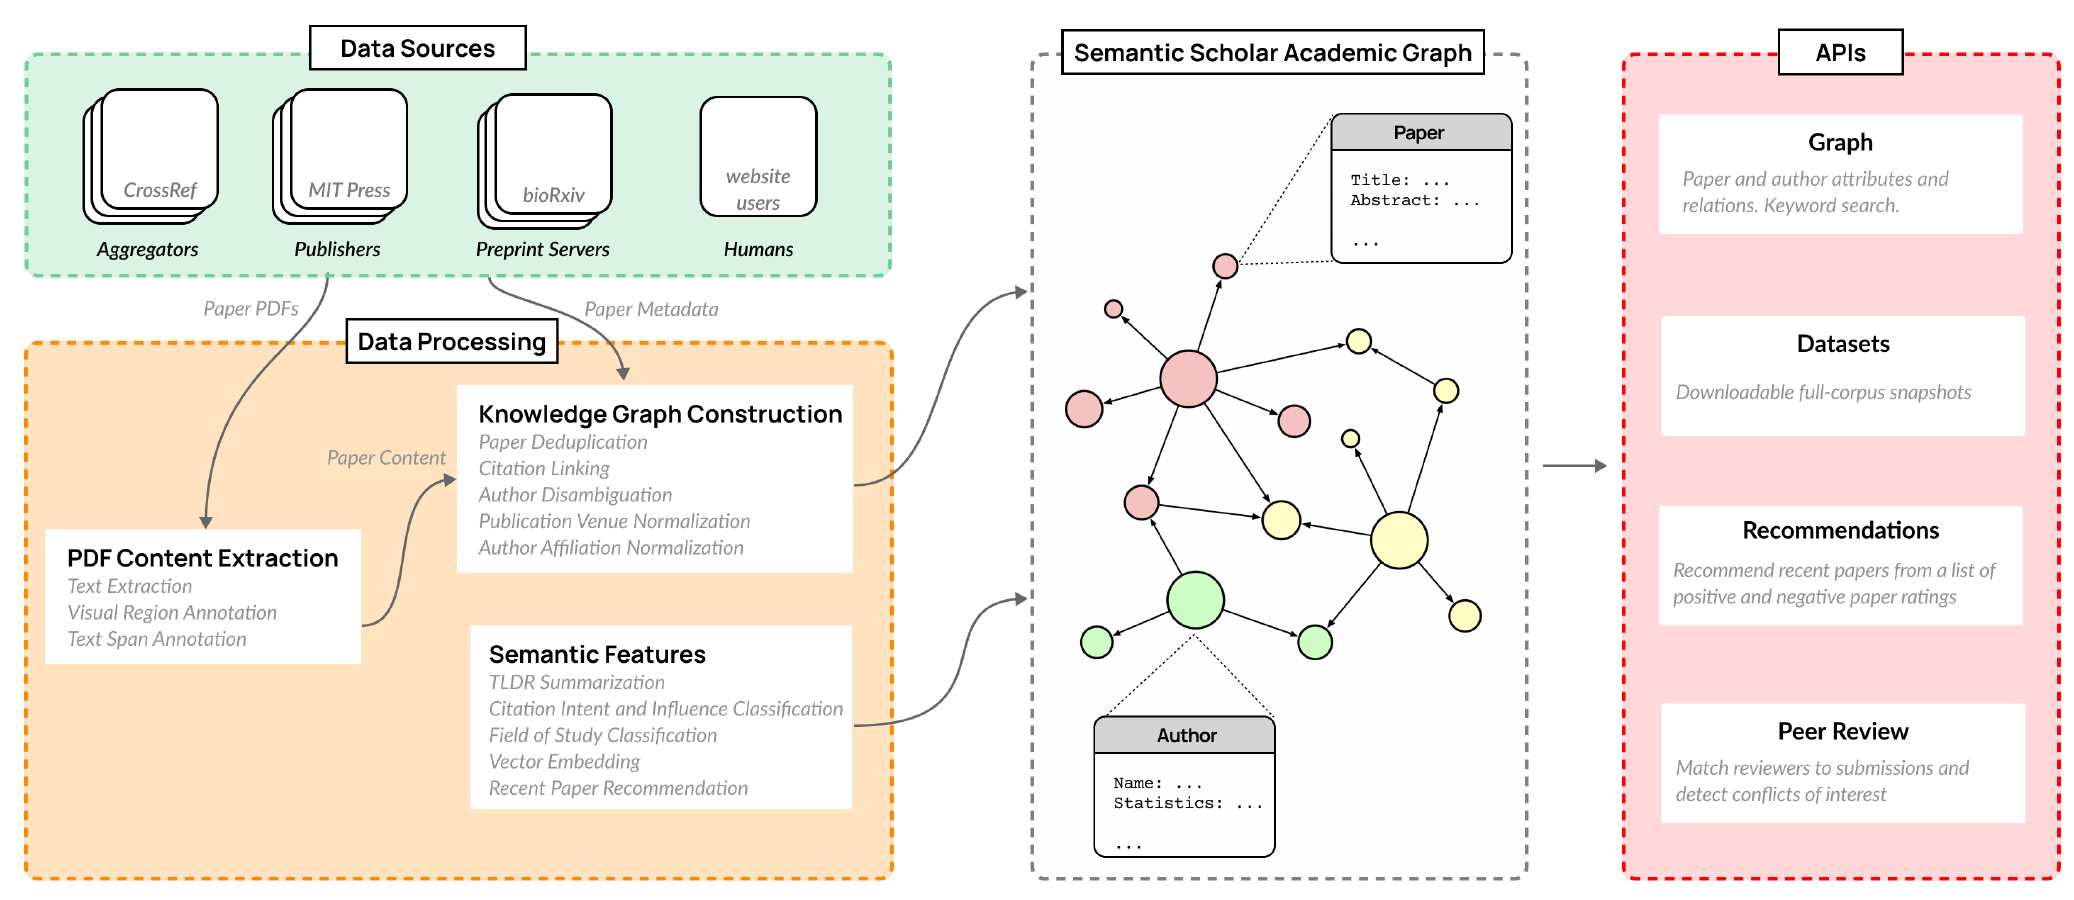
\includegraphics[width=1\textwidth,height=\textheight]{Rysunki/graf_semantic_scholar.png}
\caption{Graf platformy Semantic Scholar \label{graf_semantic_scholar}}
\end{figure}

Firma planuje w niedalekiej przyszłości udostępnić wybrane funkcje
semantyczne jako usługi, które użytkownicy będą mogli zastosować do
własnych danych oraz ulepszyć istniejącą konstrukcję grafów wiedzy i
modele cech semantycznych (\protect\hyperlink{ref-kinney2023}{Kinney i
in., 2023}).

\begin{itemize}
\tightlist
\item
  \href{lens.org}{Lens} darmowy i otwarty zasób służący do wyszukiwania,
  analizowania i zarządzania danymi patentowymi i naukowymi (rys.
  \ref{lens}). Umożliwia użytkownikom wyszukiwanie i dostęp do ponad 200
  milionów dokumentów patentowych i 100 milionów publikacji akademickich
  z różnych źródeł.
\end{itemize}

\begin{figure}
\centering

\includegraphics[width=1\textwidth,height=\textheight]{Rysunki/lens.png}
\caption{Lens \label{lens}}
\end{figure}

\begin{itemize}
\tightlist
\item
  \href{scopus.com}{Scopus}: komercyjna baza danych, której właścicielem
  jest wydawnictwo Elsevier. Zawiera ona informacje o ponad 80 milionach
  artykułów z różnych dziedzin, w tym nauk społecznych, technologii i
  opieki zdrowotnej. Indeksuje książki, czasopisma, materiały
  konferencyjne, patenty i materiały konferencyjne oraz oferuje
  użytkownikom wskaźniki cytowań, takie jak indeks h, liczba cytowań i
  efekt cytowania określonych publikacji (rys. \ref{scopus}).
\end{itemize}

\begin{figure}
\centering
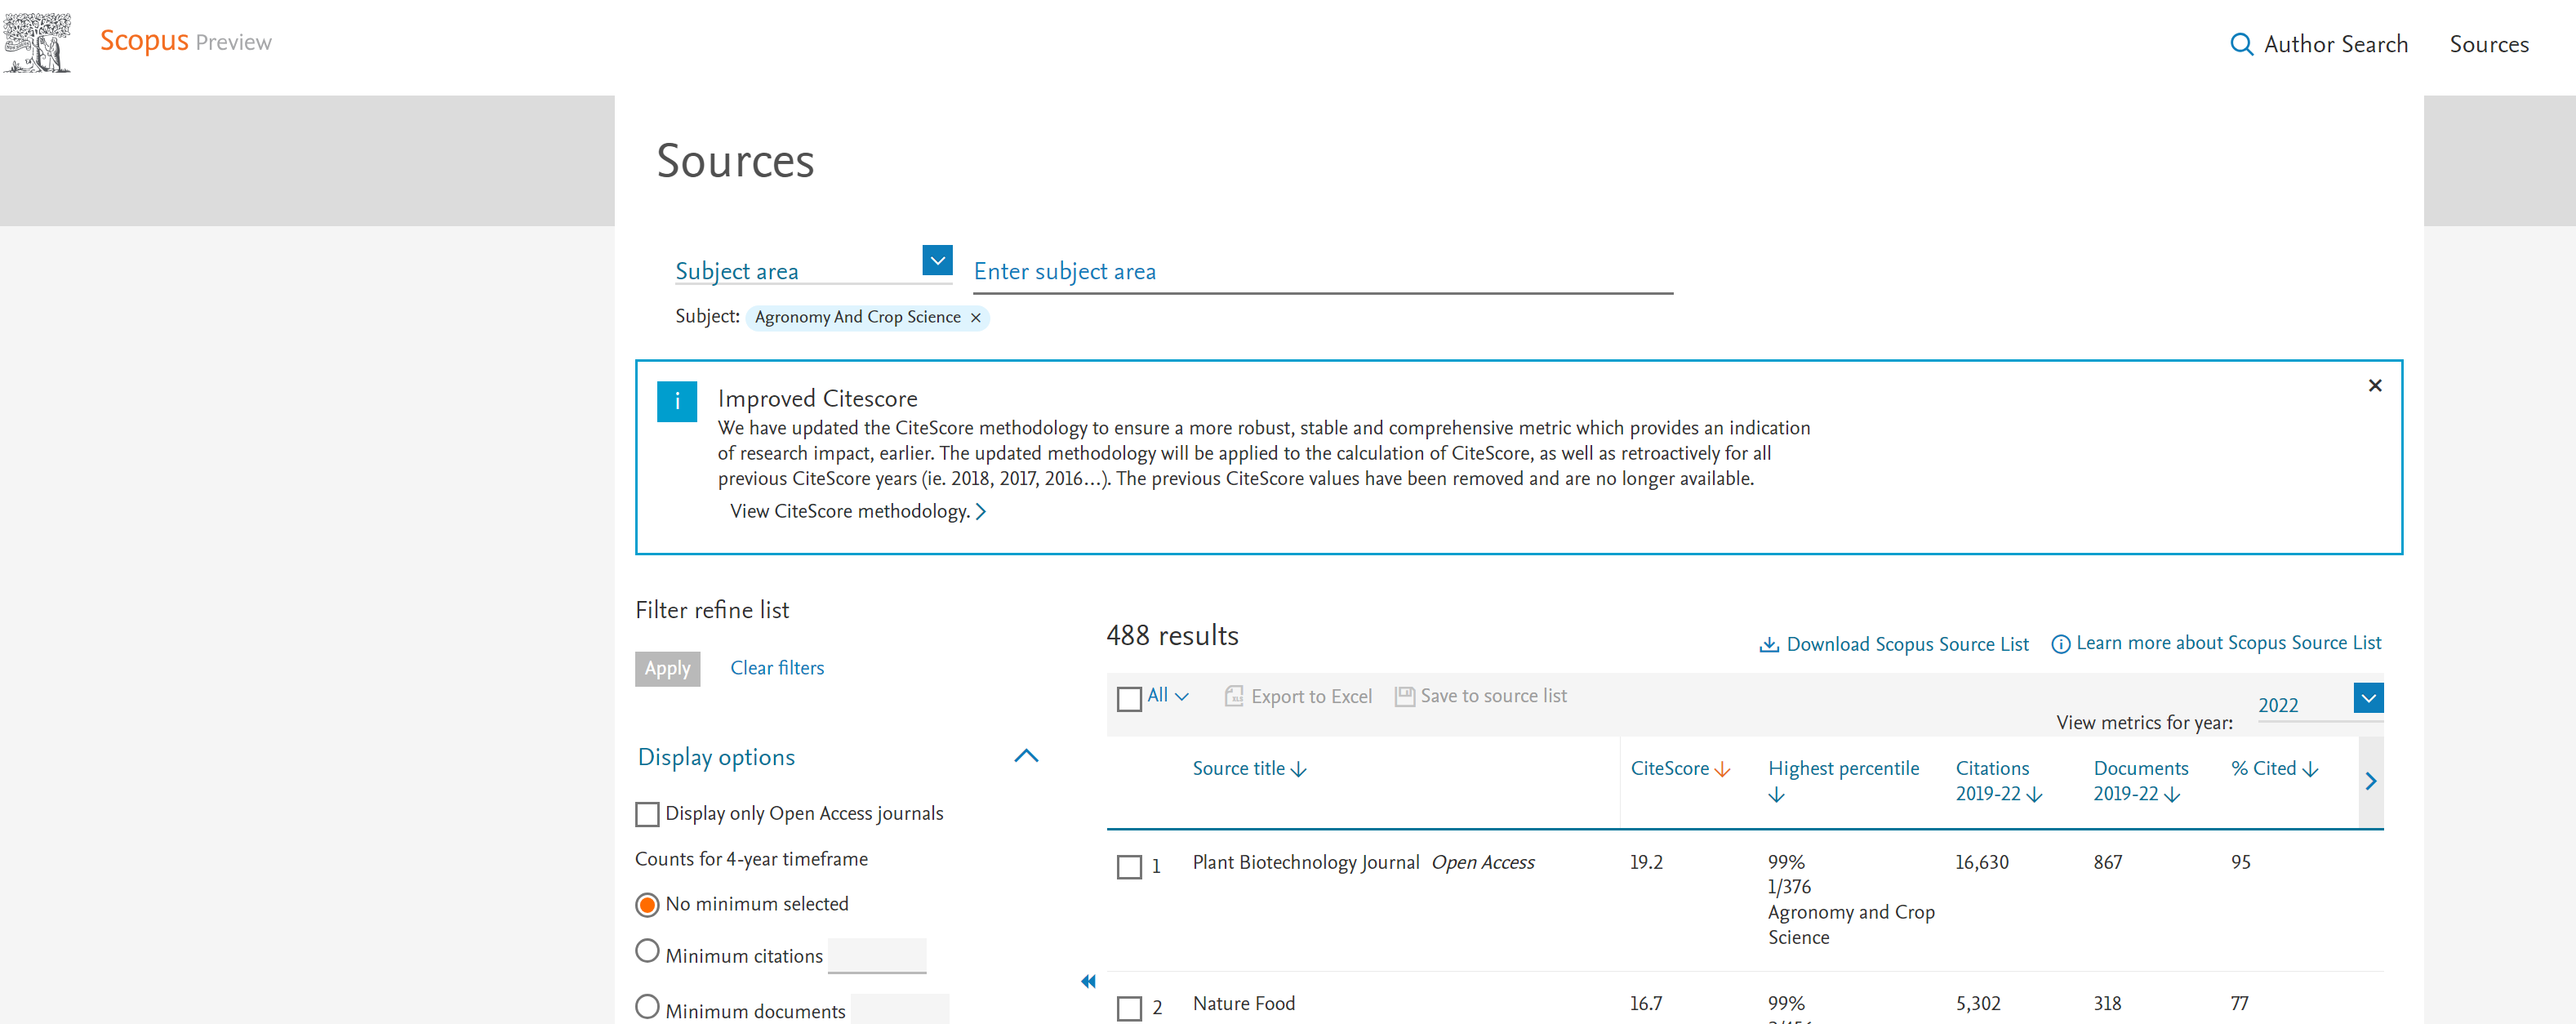
\includegraphics[width=1\textwidth,height=\textheight]{Rysunki/scopus.png}
\caption{Scopus \label{scopus}}
\end{figure}

Scopus to baza abstraktów i cytowań recenzowanej literatury, w tym
czasopism naukowych, książek i materiałów konferencyjnych. Scopus
zapewnia kompleksowy przegląd światowych wyników badań w dziedzinie nauk
ścisłych, technologii, medycyny, nauk społecznych oraz sztuki i nauk
humanistycznych.

\begin{itemize}
\tightlist
\item
  \href{webofscience.com}{Web of Science} komercyjna baza danych, której
  właścicielem jest Clarivate Analytics (rys. \ref{web_of_science}).
  Bazą danych cytowań typu for-profit, która zawiera informacje z
  zakresu nauk humanistycznych, społecznych i ścisłych. Baza danych
  zawiera recenzowane czasopisma, materiały konferencyjne, książki,
  patenty i inne publikacje naukowe, zapewniając użytkownikom dostęp do
  wiarygodnych i autorytatywnych informacji. Użytkownicy mogą przeglądać
  liczbę cytowań, indeksy h i inne wskaźniki, aby ocenić wpływ i
  znaczenie poszczególnych artykułów, autorów lub czasopism. Metodologia
  indeksowania tej bazy obejmuje proces selekcji treści, ekstrakcji
  metadanych, kontroli jakości oraz śledzenia cytowań i aktualizacji.
\end{itemize}

\begin{figure}
\centering
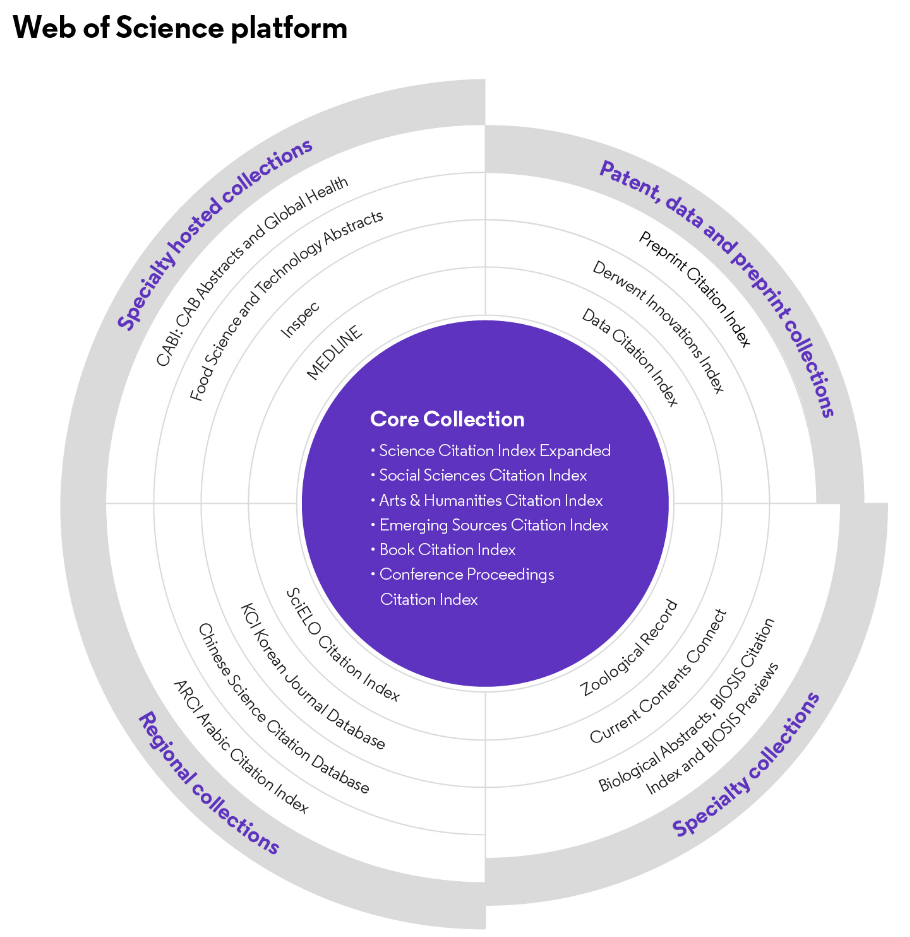
\includegraphics[width=0.7\textwidth,height=\textheight]{Rysunki/web_of_science.png}
\caption{Zakres bazy tematycznej Web of Science \label{web_of_science}}
\end{figure}

\href{researchgate.net}{ResearchGate}: ResearchGate to serwis
społecznościowy, który umożliwia naukowcom współpracę ze sobą, dzielenie
się swoją pracą i znajdowanie nowych badań (rys. \ref{researchgate}).
Ponadto oferuje użytkownikom wskaźniki cytowań, takie jak h-index,
liczba cytowań i wynik RG, który jest określany na podstawie aktywności
badawczej użytkownika na platformie.

\begin{figure}
\centering
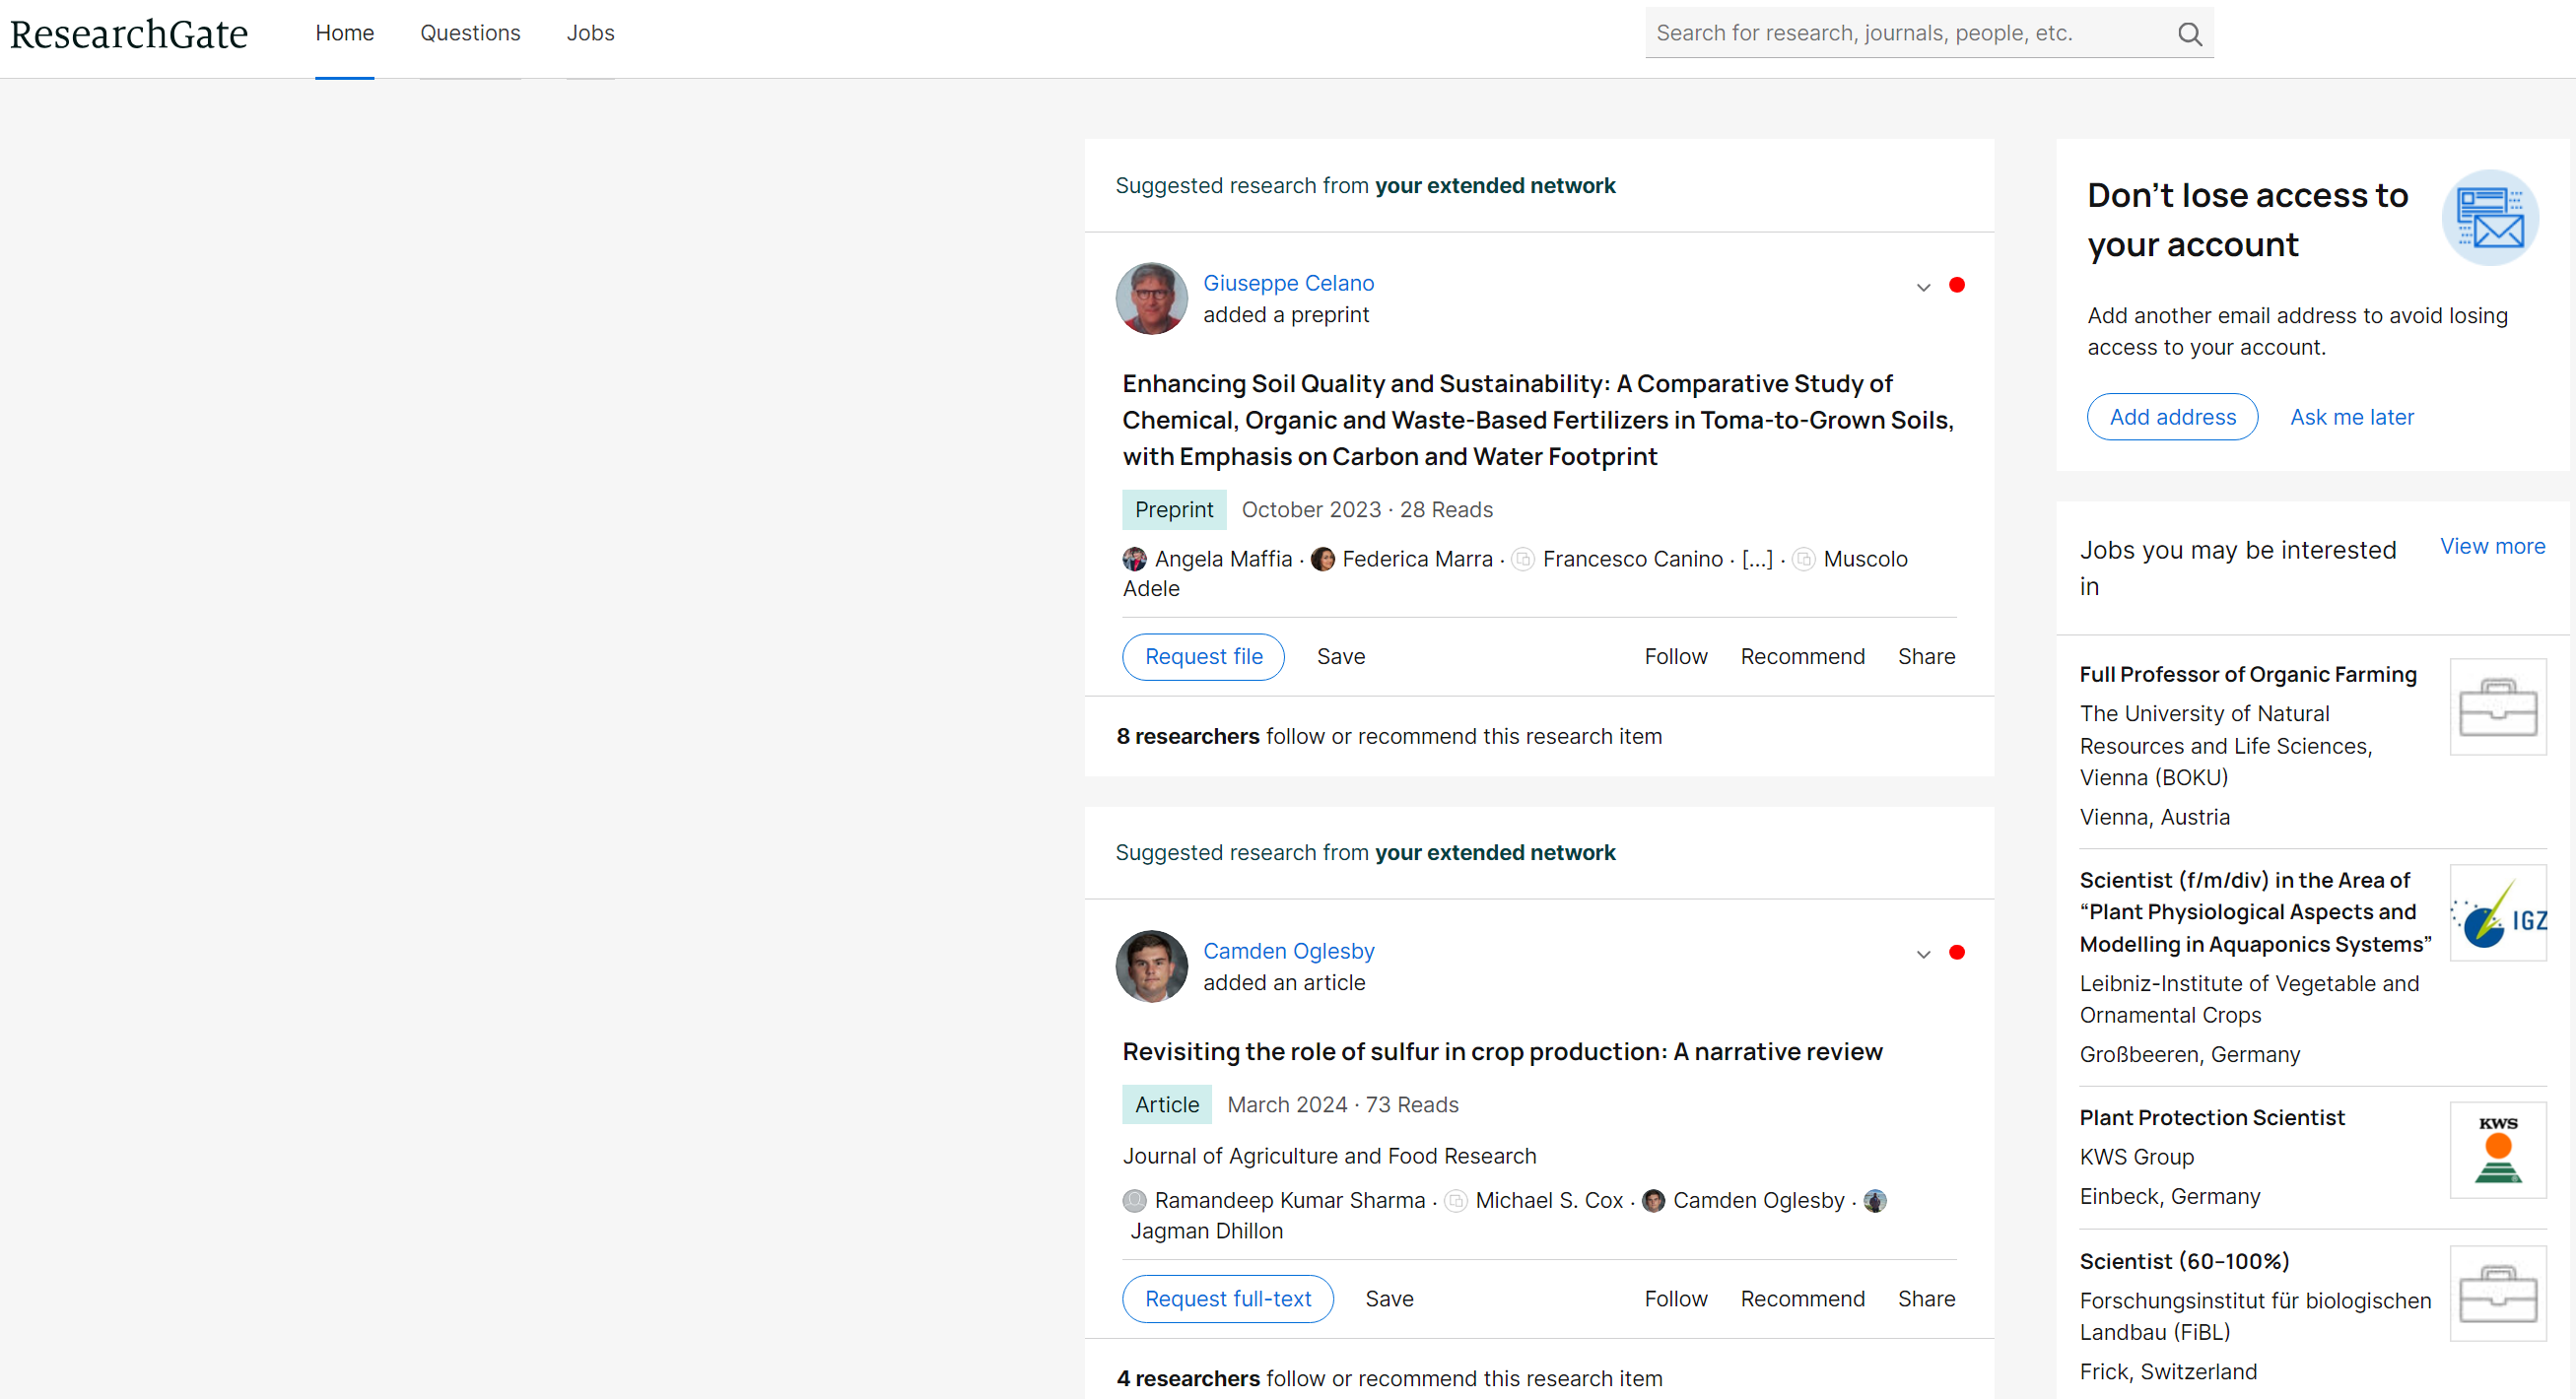
\includegraphics[width=1\textwidth,height=\textheight]{Rysunki/researchgate.png}
\caption{ResearchGate \label{researchgate}}
\end{figure}

Zestawienie głównych dostawców danych naukowych w trzech kluczowych
wymiarach: kompleksowości, dostępu i oferowanych usług przedstawiono na
rysunku \ref{bazy_biblograficzne}
(\protect\hyperlink{ref-kinney2023}{Kinney i in., 2023}). Uwidaczniają
się w tym zestawieniu duże różnice w podejściu do zakresu świadczonych
usług oraz ich dostępności. Jeden z największych dostawców tych usług
Google Scholar nie zapewnia oficjalnego dostępu API do ekstrakcji
(skrobania) danych z bazy, natomiast Semantic Scholar zapewnia
kompleksową i otwartą bazę wiedzy z najszerszym wachlarzem usług.

\begin{figure}
\centering
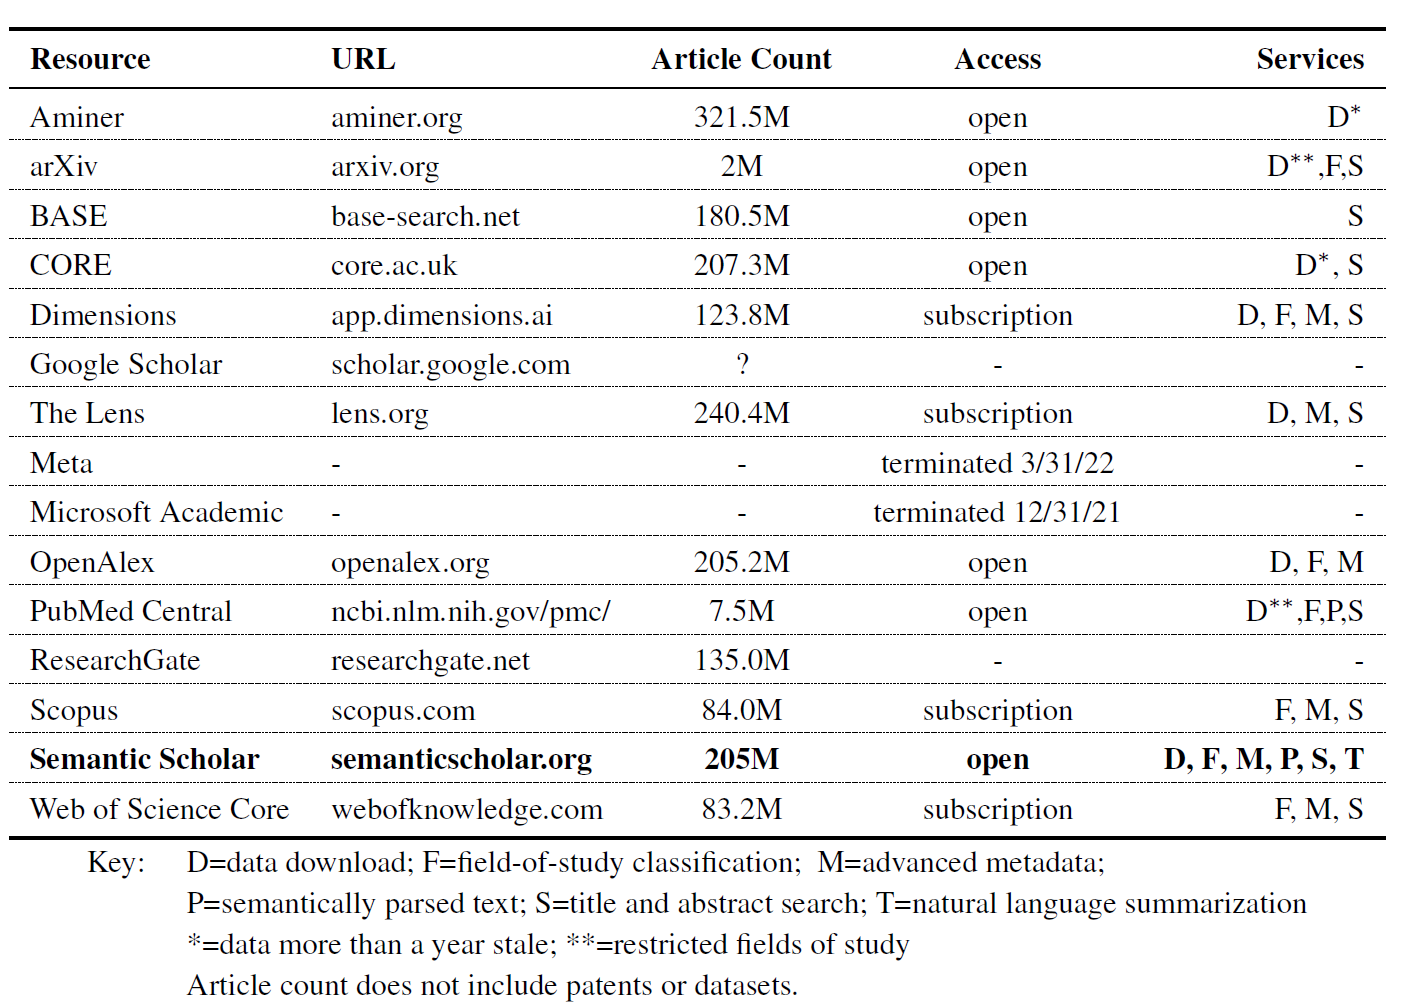
\includegraphics[width=1\textwidth,height=\textheight]{Rysunki/bazy_biblograficzne.png}
\caption{Porównanie wiodących dostawców danych naukowych
\label{bazy_biblograficzne}}
\end{figure}

\textbf{Podsumowanie:}

Na podstawie powyższego opisu uwidacznia się wyraźnie problem z
wyszukaniem najlepiej powiązanych artykułów naukowych dla zakładanego
tematu badań. Wykonywanie takich przeglądów standardowymi ``ręcznymi''
metodami jest bardzo czasochłonne i mało efektywne, dlatego metody i
narzędzia data science umożliwiają ten etap pracy naukowej znacznie
przyspieszyć i zwiększyć jego efektywność.

\FloatBarrier
\newpage
\fancyhead[C]{Metodyka badań}

\hypertarget{metody-badaux144}{%
\section{Metody badań}\label{metody-badaux144}}

W pracy własnej wykorzystano narzędzia z obszaru dziedziny Data Science,
dlatego poniżej zdefiniowano ten obszar wiedzy.

\textbf{Data Science} (polska nazwa - danologia) to interdyscyplinarna
dziedzina generalnie zajmująca się analizą danych (pozyskiwaniem,
eksploracją, wizualizowaniem i wyciąganiem z takich analiz wniosków. W
szeroko rozumianym obszarze Data Science wykorzystuje się metody oparte
na programowaniu, analizie statystycznej, analizie dużych baz danych
(Big Data) oraz metody z zakresu sztucznej inteligencji, czyli uczenie
maszynowe (Machine Learning), czy sieci neuronowe.

\hypertarget{narzux119dzia-data-science-wykorzystane-w-pracy}{%
\subsection{Narzędzia Data Science wykorzystane w
pracy}\label{narzux119dzia-data-science-wykorzystane-w-pracy}}

\begin{itemize}
\tightlist
\item
  Program Python
\item
  Program R
\item
  Program LaTeX
\item
  RStudio
\item
  R Markdown
\item
  Zotero menadżer biblografii.
\end{itemize}

\hypertarget{program-python-python.org}{%
\subsubsection{\texorpdfstring{Program Python
\href{https://www.python.org}{python.org}}{Program Python python.org}}\label{program-python-python.org}}

Python określany jest jako wysoko poziomowy, dynamiczny językiem
ogólnego przeznaczenia (rys. \ref{python}).

\begin{figure}
\centering

\includegraphics[width=0.8\textwidth,height=\textheight]{Rysunki/python.png}
\caption{Program Python \label{python}}
\end{figure}

Obecnie jest najbardziej popularnym i najszybciej rozwijającym się
językiem programowania na świecie według portalu
\href{https://www.tiobe.com/tiobe-index/}{TIOBE Index} (rys.
\ref{ranking_prog}).

\begin{figure}
\centering
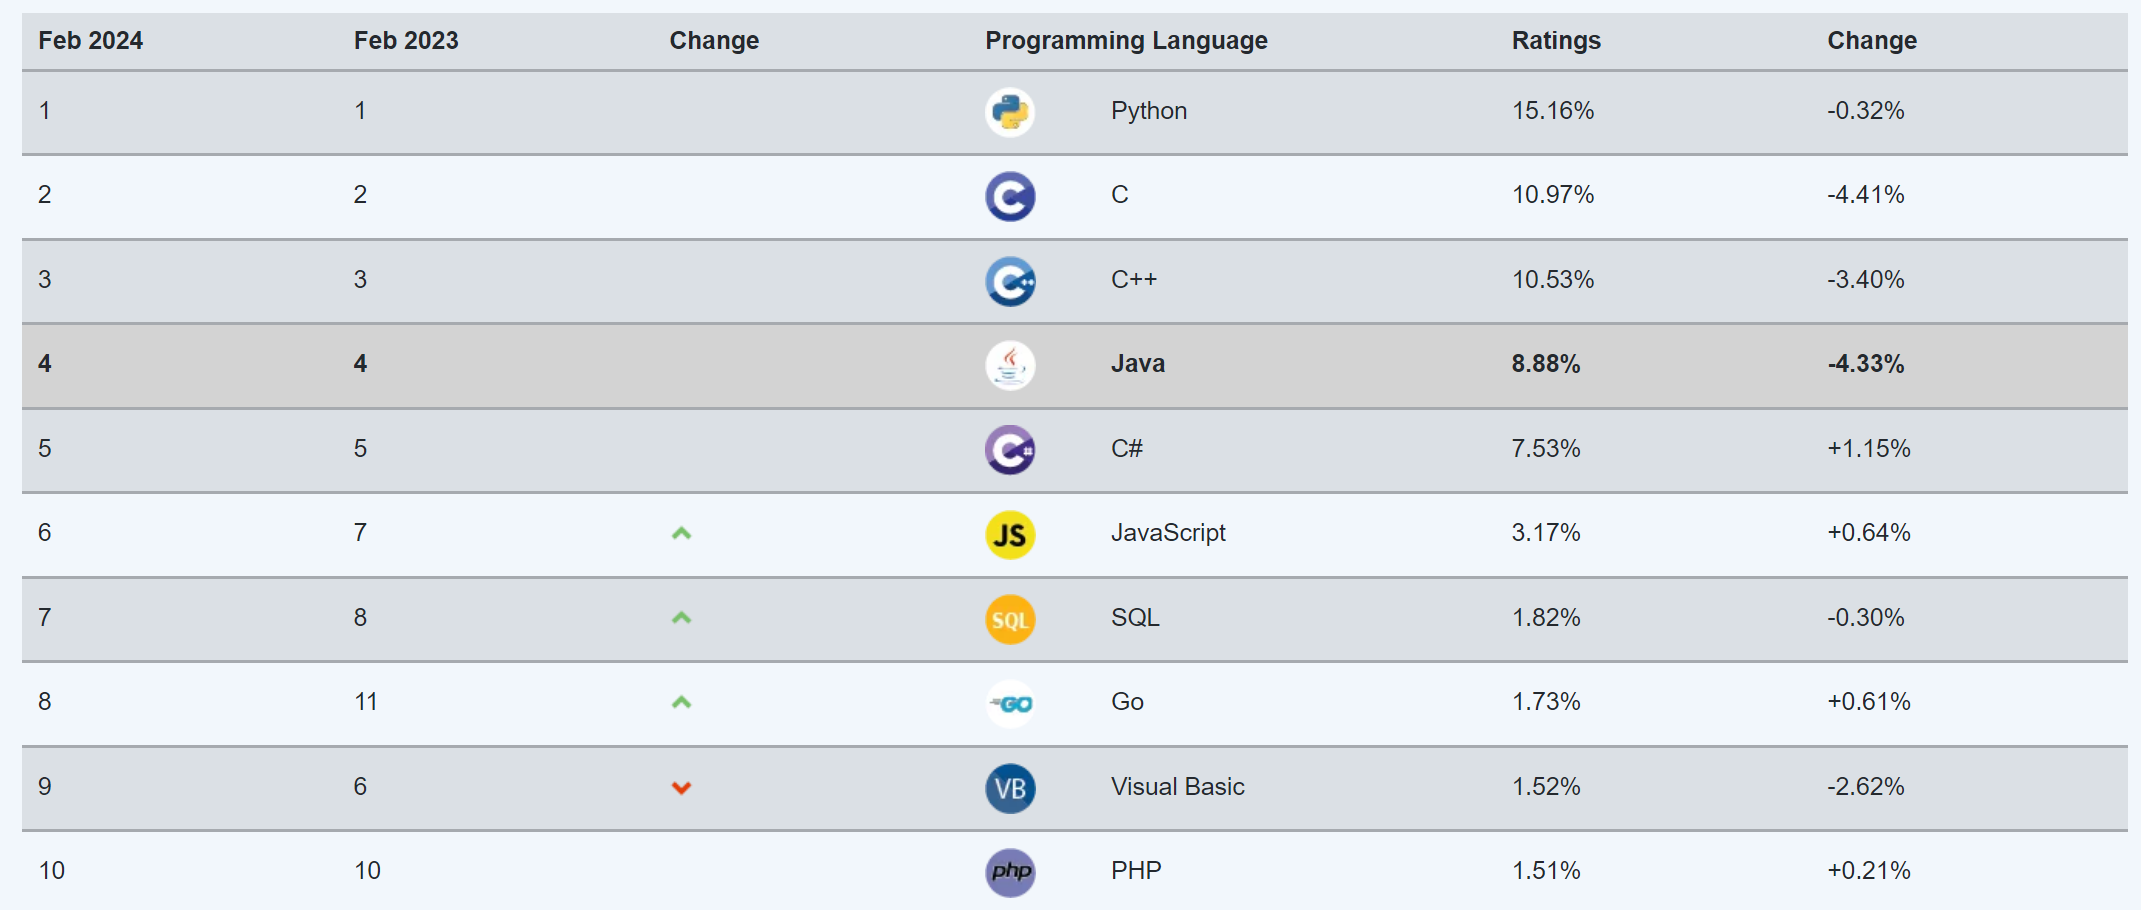
\includegraphics[width=1\textwidth,height=\textheight]{Rysunki/ranking_programow.png}
\caption{Ranking programów TIOBE Index \label{ranking_prog}}
\end{figure}

Pierwsza wersja Pythona ukazała się na początku 1991 roku i zaliczany
jest do kategorii oprogramowania Open Source. Do głównych zalet Pythona
zalicza się nowoczesną składnię języka z opcją wyboru różnych
paradygmatów programowania (funkcyjnego, obiektowego, reaktywnego), dużą
i przyjazną społeczność, bogaty zbiór wbudowanych i przenośnych opcji,
sprawną komunikację z innymi częściami aplikacji, współpracę pomiędzy
najważniejszymi platformami - Windowsa oraz Linuxa
(\protect\hyperlink{ref-comarch2023}{Comarch, 2023}).

\hypertarget{program-r-r-project.org}{%
\subsubsection{\texorpdfstring{Program R
\href{https://www.r-project.org}{r-project.org}}{Program R r-project.org}}\label{program-r-r-project.org}}

R jest oprogramowaniem o otwartym kodzie źródłowym, dostępnym w Uniksie,
Linuksie, a także systemach macOS i Windows
(\protect\hyperlink{ref-wickham2018}{Wickham i Grolemund, 2018}).

Logo tego programu przedstawiono na rysunku \ref{r_logo.svg}.

\begin{figure}
\centering

\includegraphics[width=0.2\textwidth,height=\textheight]{Rysunki/r_logo_svg.png}
\caption{Logo programu R. \label{r_logo.svg}}
\end{figure}

Język R jest językiem interpretowanym z elastyczną składnią i pozwala
użytkownikom na definiowanie własnych, dowolnie złożonych, funkcji
(\protect\hyperlink{ref-guxf3recki2011}{Górecki, 2011}).

R wykorzystuje się do obliczeń statystyczno-matematycznych, umożliwia on
również tworzenie zaawansowanych wykresów.

Po zainstalowaniu podstawowego środowiska R mamy już dostęp do wielu
użytecznych funkcjonalności, jednak możliwości pracy w R zwiększają się
bardzo po zainstalowaniu dodatkowych pakietów (package). Szacuje się, że
2020 roku dostępnych ich było około 16 tysięcy
\href{https://en.wikipedia.org/wiki/R_package}{wikipedia.org}.

\hypertarget{rstudio-rstudio.com}{%
\subsubsection{\texorpdfstring{RStudio
\href{https://www.rstudio.com}{rstudio.com}}{RStudio rstudio.com}}\label{rstudio-rstudio.com}}

Istnieje kilka graficznych interfejsów dla programu R, wśród nich
najbardziej popularnym jest RStudio (rys. \ref{rstudio}).

RStudio określa się jako zintegrowane środowisko programistyczne (IDE)
dla języka R.

\begin{figure}
\centering

\includegraphics[width=0.3\textwidth,height=\textheight]{Rysunki/r_studio.png}
\caption{Logo RStudio\label{rstudio}}
\end{figure}

RStudio zawiera konsolę, edytor podświetlający składnię i obsługuje
bezpośrednie wykonywanie kodu, a także narzędzia do tworzenia wykresów,
historii, debugowania i zarządzania przestrzenią roboczą (rys.
\ref{rstudio_edytor}).

\begin{figure}
\centering
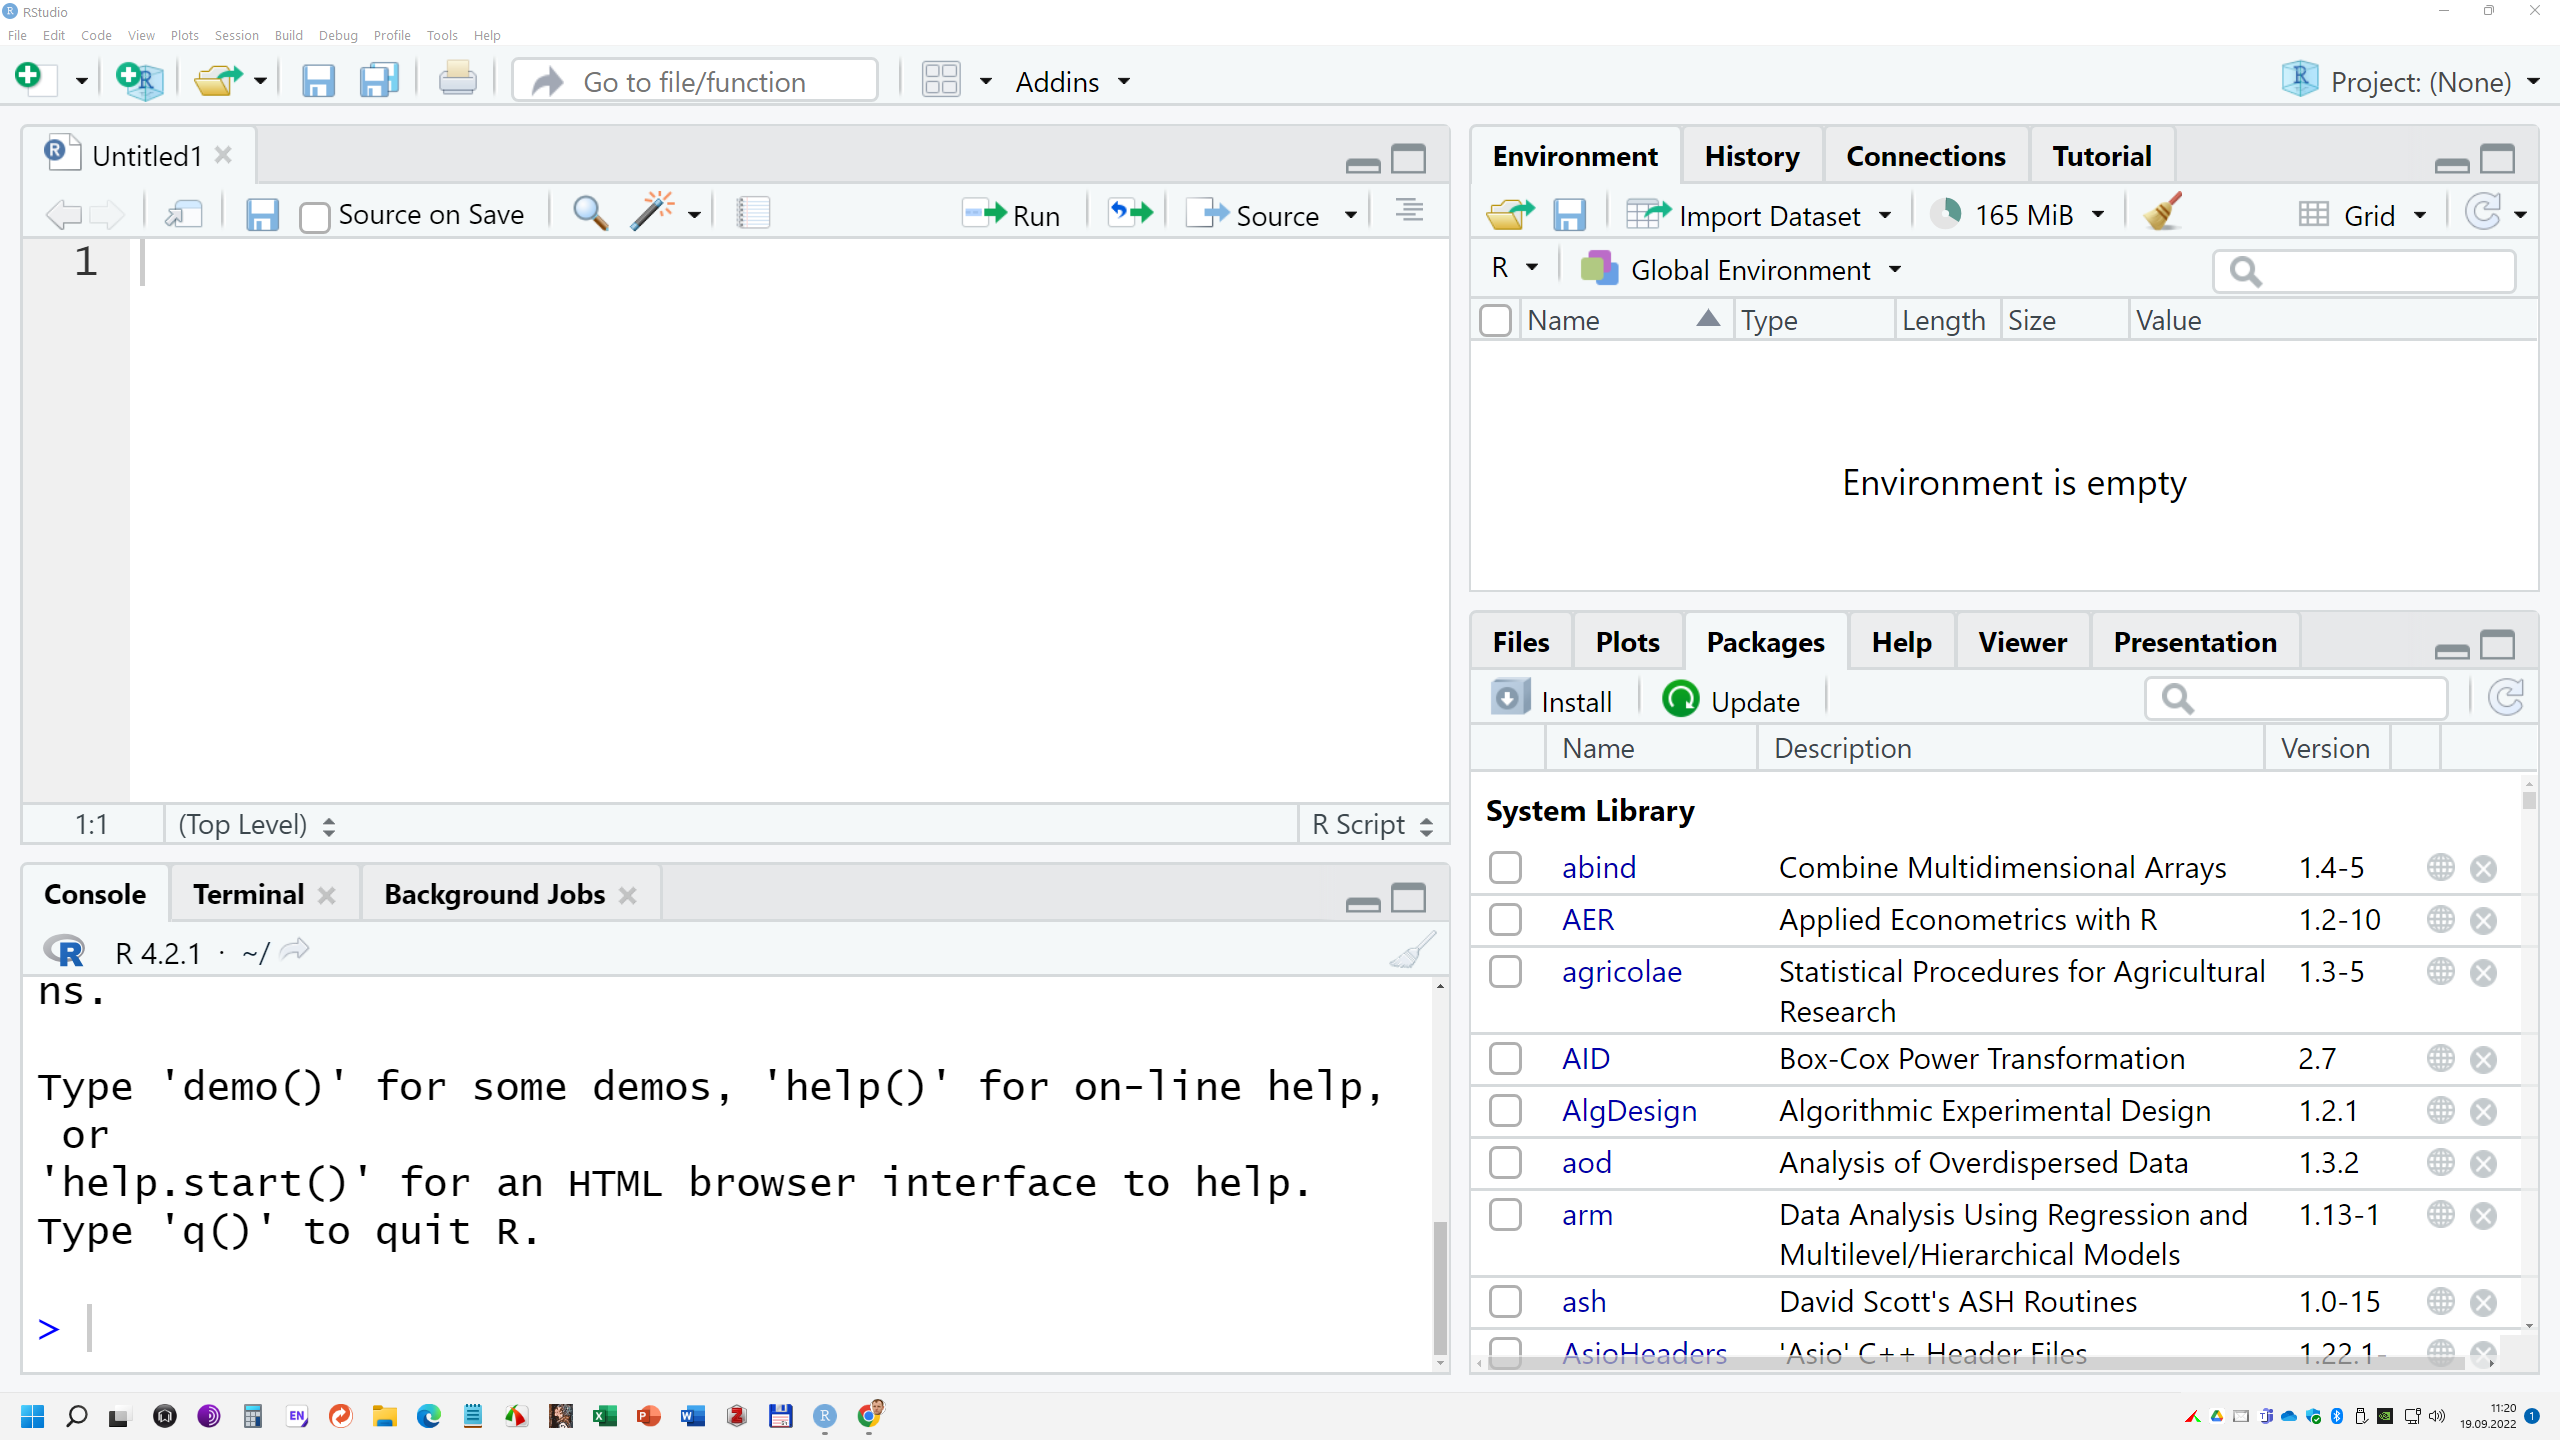
\includegraphics{Rysunki/rstudio_edytor.png}
\caption{RStudio\label{rstudio_edytor}}
\end{figure}

\hypertarget{r-markdown-rmarkdown.com}{%
\subsubsection{\texorpdfstring{R Markdown
\href{https://rmarkdown.rstudio.com/}{rmarkdown.com}}{R Markdown rmarkdown.com}}\label{r-markdown-rmarkdown.com}}

Rmarkdown to narzędzie do tworzenia dynamicznych dokumentów i zestawień.
Język znaczników, którego celem jest jak największe uproszczenie
tworzenia i formatowania tekstu
\href{https://en.wikipedia.org/wiki/Markdown}{wikipedia.org}.

\begin{figure}
\centering

\includegraphics[width=0.4\textwidth,height=\textheight]{Rysunki/r_markdown.png}
\caption{Rmarkdown \label{rmarkdown}}
\end{figure}

Biblioteka rmarkdown wraz z formatem R Markdown pozwala na przygotowanie
estetycznie wyglądających raportów, a dokumenty otrzymywane w wyniku ich
tworzenia są dynamiczne ponieważ istnieje w nich możliwość zagnieżdżania
języka R (\protect\hyperlink{ref-strus2017}{Struś, 2017}).

\hypertarget{latex-latex-project.org}{%
\subsubsection{\texorpdfstring{LaTeX
\href{https://www.latex-project.org/}{latex-project.org}}{LaTeX latex-project.org}}\label{latex-latex-project.org}}

LaTeX to oprogramowanie do zautomatyzowanego składu tekstu, a także
związany z nim język znaczników, służący do formatowania dokumentów
tekstowych i tekstowo-graficznych
\href{https://pl.wikipedia.org/wiki/LaTeX}{wikipedia.org}.

\begin{figure}
\centering

\includegraphics[width=0.4\textwidth,height=\textheight]{Rysunki/LaTeX.png}
\caption{LaTeX\label{latex}}
\end{figure}

Oprogramowanie to określane jest także jako zestaw makropoleceń
stanowiących nadbudowę nad systemem składu TEX, automatyzujących wiele
czynności związanych z procesem poprawnego składania tekstu
(\protect\hyperlink{ref-ziemkiewicz2013}{Ziemkiewicz i Karłowska-Pik,
2013}).

\hypertarget{wybuxf3r-baz-danych-indeksujacych-publikacje-naukowe}{%
\subsection{Wybór baz danych indeksujacych publikacje
naukowe}\label{wybuxf3r-baz-danych-indeksujacych-publikacje-naukowe}}

Do badań własnych z zakresu przeglądu literatury naukowej wybrano dwie
różniące się wieloma cechami bazy danych: \textbf{Google Scholar} oraz
\textbf{Semantic Scholar}.

Przyjęto \textbf{metodę bibliometrycznego przeglądu literatury}, czyli
oceniano literaturę w systematyczny sposób poprzez pomiar (ilościowy)
określonych wskaźników dla autorów publikacji, ilości ich cytowań,
rodzaju czasopism, czy lata publikacji).

W przeciwieństwie do przeglądów tradycyjnych, charakterystyką metody
przeglądu bibliometrycznego jest to, że cały proces pozyskiwania, oceny
i syntezy literatury powinien być dokładnie dokumentowany i przebiegać
według ściśle określonych standardów
(\protect\hyperlink{ref-tranfield2003}{Tranfield i in., 2003}).

\FloatBarrier
\newpage
\fancyhead[C]{Wyniki analiz}

\hypertarget{wyniki-badaux144-i-analiz}{%
\section{Wyniki badań i analiz}\label{wyniki-badaux144-i-analiz}}

\hypertarget{baza-danych-google-scholar-gs}{%
\subsection{Baza danych Google Scholar
(GS)}\label{baza-danych-google-scholar-gs}}

Przeszukiwanie bazy w tradycyjny sposób odbywa się poprzez wyszukiwarkę
strony \href{https://scholar.google.com}{Google Scholar}.

\begin{Shaded}
\begin{Highlighting}[]
\FunctionTok{library}\NormalTok{(webshot2)}
\FunctionTok{webshot}\NormalTok{(}\StringTok{"https://scholar.google.com"}\NormalTok{, }
        \StringTok{"Rysunki/wyszykiwarka\_google\_scholar.png"}\NormalTok{)}
\end{Highlighting}
\end{Shaded}


\includegraphics{Rysunki/figures/unnamed-chunk-27-1.png}

Przeszukiwanie zasobów GS różni się pod kilkoma względami od
przeszukiwania innych baz. Baza ta posiada własną listę operatorów,
które nie występują w żadnej innej bazie danych. Stosować można podczas
wyszukiwania niektóre popularne operatory ograniczające lub
rozszerzające wyszukiwanie (takie jak cudzysłów lub gwiazdka), natomiast
z innych jak operatora wyszukiwania logicznego NOT nie można skorzystać.
Google używa znaku minus zamiast powszechnie używanego terminu NOT. GS
używają niejawnego AND - a nie logicznego AND, czyli kiedy operator ten
jest wprowadzane do zapytania wyszukiwania, Google traktuje je jako
słowo w zapytaniu wyszukiwania i nie rozpoznaje go jako operatora
wyszukiwania. GS ignoruje popularne słowa, takie jak a, and, the i tak
dalej, z wyjątkiem gdy umieszczone są w cudzysłowie.

\textbf{Wybrane operatory wyszukiwania Google Scholar:}

\textbf{publikacja:} Wyniki będą zawierać tylko publikacje zawierające
określone terminy. Na przykład wyszukiwanie ``publication:computers in
libraries'' będzie zawierać tylko wyniki z publikacji Computers in
Libraries.

\textbf{autor:} Lista wyników będzie zawierać tylko publikacje
wskazanego autora, na przykład, autor: G Kulczycki

\textbf{define:} używany tylko w Google, gdy oczekuje się szybkich
definicji, na przykład, ``define:word''

\textbf{cudzysłów ('' ``)} używany do łączenia dokładnej frazy, może być
również używany do zapewnienia, że określone słowo zostanie
uwzględnione.

\textbf{Uniwersalne operatory logiczne i logika wyszukiwania:}

\textbf{OR} - znany również jako suma logiczna, operator OR ``rozszerza
wyszukiwanie poprzez uwzględnienie synonimów i powiązanych terminów w
zapytaniu''

\textbf{znak minus (-)} główną funkcją znaku minus jest wykluczenie
terminu, GS używa znaku minus zamiast powszechnie używanego terminu NOT.

\textbf{gwiazdka (*)} używana jako operator wieloznaczny

Przykład wyszukiwania w basie GS dla frazy ``elemental sulphur
fertilization'' w wyniku wyszukiwania uzyskuje się 42 pozycje publikacji
(rys. \ref{GS_elemental}).

\begin{figure}
\centering
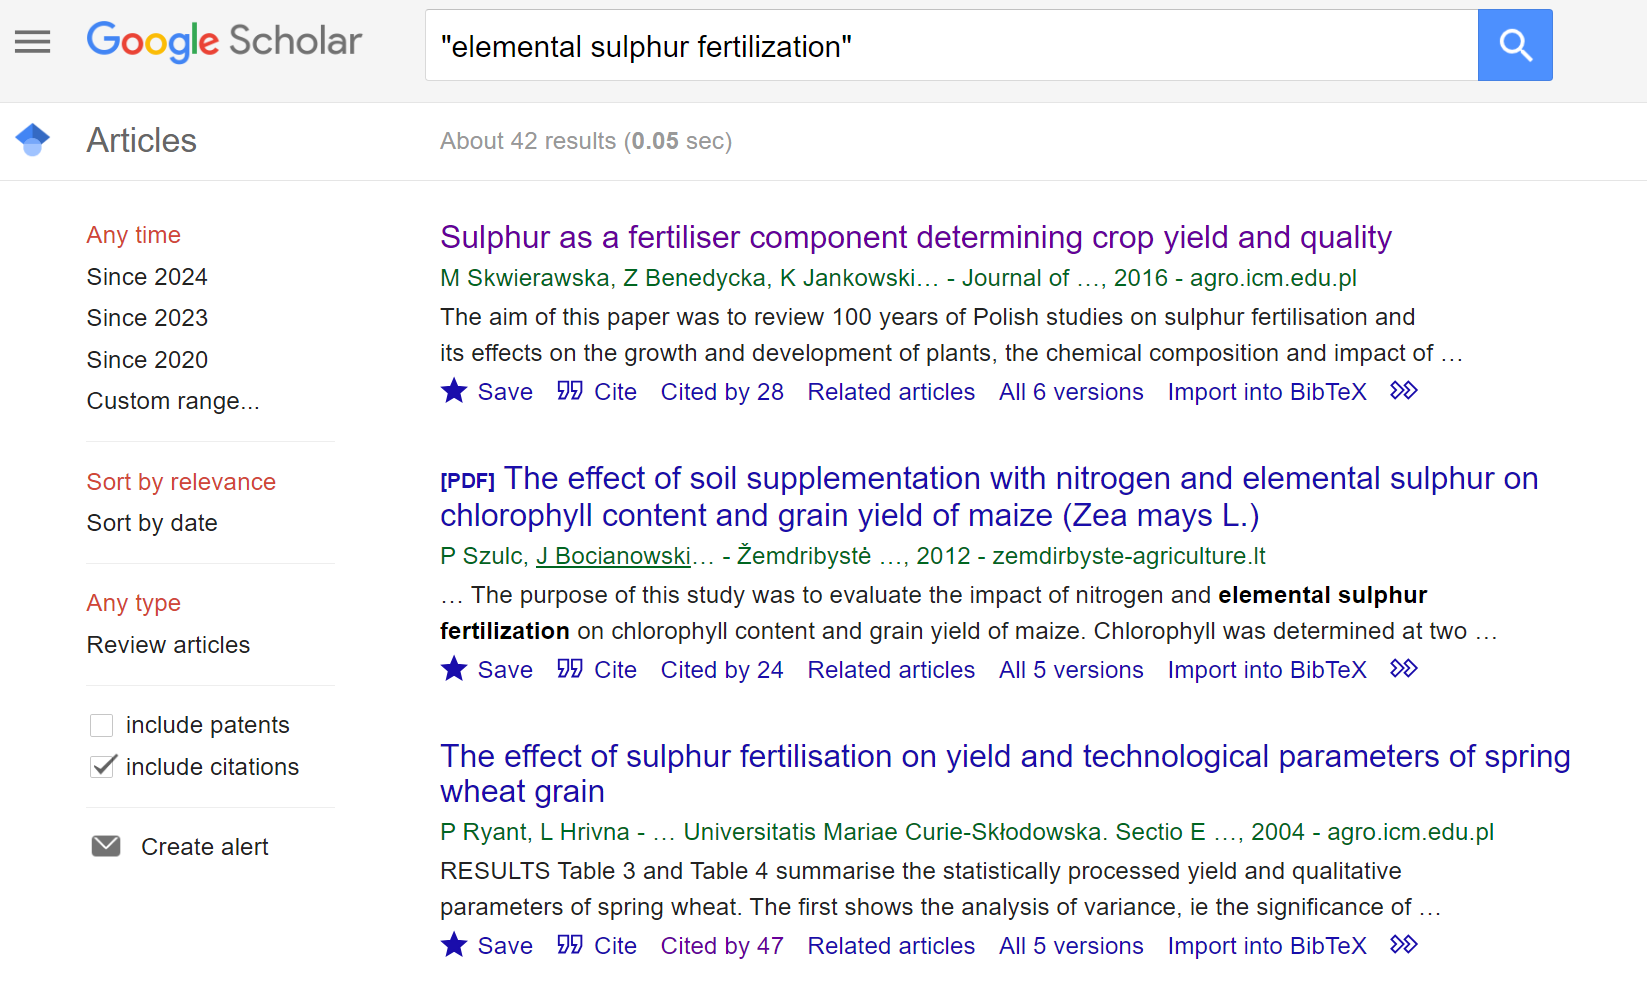
\includegraphics[width=1\textwidth,height=\textheight]{Rysunki/wyniki_wyszukiwania/GS_elemental_sulphur_fertilization.png}
\caption{Wyszukiwanie tradycyjne frazy słów w GS \label{GS_elemental}}
\end{figure}

\href{https://policies.google.com/terms/archive/20190122?hl=en&gl=GB}{Polityka
firmy Google} określa, że dostęp do zasobów GS powinien odbywać poprzez
interfejs ich wyszukiwarki i instrukcji podanych przez firmę. GS nie
zapewnia API (Application Programming Interface), a dostęp do zasobów
jest wyszczególniony poprzez plik robot.txt.

\begin{Shaded}
\begin{Highlighting}[]
\FunctionTok{library}\NormalTok{(webshot2)}
\FunctionTok{webshot}\NormalTok{(}\StringTok{"https://scholar.google.com/robots.txt"}\NormalTok{, }\StringTok{"Rysunki/robots.png"}\NormalTok{) }
\end{Highlighting}
\end{Shaded}

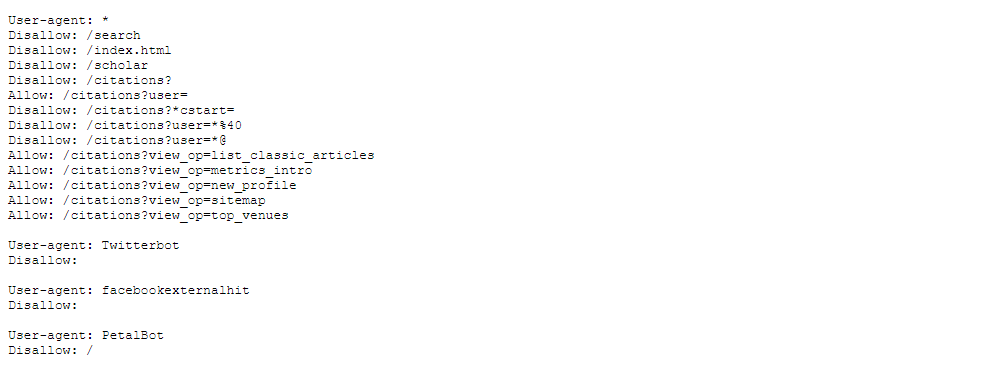
\includegraphics{Rysunki/figures/unnamed-chunk-28-1.png}

\textbf{Baza Google Scholar zezwala na dostęp do:}

\begin{itemize}
\tightlist
\item
  profili użytkowników: Allow: /citations?user=
\end{itemize}

(np.
\href{https://scholar.google.pl/citations?user=RNDE9-wAAAAJ&hl=pl}{https://scholar.google.pl/citations?user=RNDE9-wAAAAJ\&hl})

\begin{itemize}
\tightlist
\item
  zestawienia bbszarów dziedzin badawczych: Allow:
  /citations?view\_op=list\_classic\_articles
\end{itemize}

(np.
\url{https://scholar.google.com/citations?view_op=list_classic_articles&hl=en&by=2006})

\begin{itemize}
\tightlist
\item
  Zeztawienia kategorii czasopism: Allow:
  /citations?view\_op=metrics\_intro
\end{itemize}

(np. \url{https://scholar.google.com//citations?view_op=metrics_intro})

\hypertarget{analiza-wskaux17anikuxf3w-biblometrycznych-dla-wybranych-naukowcuxf3w}{%
\subsubsection{Analiza wskaźników biblometrycznych dla wybranych
naukowców}\label{analiza-wskaux17anikuxf3w-biblometrycznych-dla-wybranych-naukowcuxf3w}}

W ramach dozwolonego przez GS dostępu do bazy przeprowadzono analizę
wskaźników bibliometrycznych dla wybranych naukowców za pomocą
biblioteki
\href{https://cran.r-project.org/web/packages/scholar/index.html}{scholar}.

\hypertarget{analiza-iloux15bci-publikacji}{%
\subsubsection{Analiza ilości
publikacji}\label{analiza-iloux15bci-publikacji}}

\begin{Shaded}
\begin{Highlighting}[]
\CommentTok{\#wymagane bibloteki}
\FunctionTok{library}\NormalTok{(scholar)}
\FunctionTok{library}\NormalTok{(tidyverse)}
\FunctionTok{library}\NormalTok{(ggplot2)}

\CommentTok{\# id  użytkowników}
\NormalTok{Kulczycki }\OtherTok{\textless{}{-}} \StringTok{"RNDE9{-}wAAAAJ\&hl"}  
\NormalTok{Sacala }\OtherTok{\textless{}{-}} \StringTok{"jkj3pCQAAAAJ\&hl"} 
\NormalTok{Lejcus }\OtherTok{\textless{}{-}} \StringTok{"XNRUNHsAAAAJ\&hl"} 
\NormalTok{Pietr }\OtherTok{\textless{}{-}} \StringTok{"L6MYKCQAAAAJ\&hl"} 

\CommentTok{\# Ile artykułów opublikowali?}
\NormalTok{Kulczycki.num }\OtherTok{\textless{}{-}} \FunctionTok{get\_num\_articles}\NormalTok{(Kulczycki)}
\NormalTok{Sacala.num }\OtherTok{\textless{}{-}} \FunctionTok{get\_num\_articles}\NormalTok{(Sacala)}
\NormalTok{Lejcus.num }\OtherTok{\textless{}{-}} \FunctionTok{get\_num\_articles}\NormalTok{(Lejcus)}
\NormalTok{Pietr.num }\OtherTok{\textless{}{-}} \FunctionTok{get\_num\_articles}\NormalTok{(Pietr)}

\CommentTok{\# utworzenie ramki danych}
\NormalTok{num }\OtherTok{\textless{}{-}} \FunctionTok{data.frame}\NormalTok{ (}\AttributeTok{Ilosc =} \FunctionTok{c}\NormalTok{(Kulczycki.num, }
\NormalTok{                              Sacala.num, }
\NormalTok{                              Lejcus.num, }
\NormalTok{                              Pietr.num),}
                  \AttributeTok{Osoba=} \FunctionTok{c}\NormalTok{(}\StringTok{"Kulczycki"}\NormalTok{, }\StringTok{"Sacala"}\NormalTok{, }\StringTok{"Lejcus"}\NormalTok{, }\StringTok{"Pietr"}\NormalTok{))}

\CommentTok{\# wizualizacja ilości cytowań}
\FunctionTok{ggplot}\NormalTok{(num, }\FunctionTok{aes}\NormalTok{(}\AttributeTok{x=}\NormalTok{Osoba, }\AttributeTok{y=}\NormalTok{Ilosc, }\AttributeTok{col =}\NormalTok{ Ilosc, }\AttributeTok{fill =}\NormalTok{ Osoba)) }\SpecialCharTok{+} 
\FunctionTok{geom\_col}\NormalTok{()}\SpecialCharTok{+}
\FunctionTok{theme\_bw}\NormalTok{() }\SpecialCharTok{+} 
\FunctionTok{scale\_fill\_brewer}\NormalTok{(}\AttributeTok{palette =} \StringTok{"BrBG"}\NormalTok{)}\SpecialCharTok{+}
\FunctionTok{geom\_text}\NormalTok{(}\FunctionTok{aes}\NormalTok{(}\AttributeTok{label=}\NormalTok{Ilosc),}\AttributeTok{position=}\FunctionTok{position\_stack}\NormalTok{(}\AttributeTok{vjust=}\FloatTok{1.1}\NormalTok{),}\AttributeTok{size=}\DecValTok{8}\NormalTok{)}\SpecialCharTok{+}
\FunctionTok{theme}\NormalTok{( }\AttributeTok{plot.title =} \FunctionTok{element\_text}\NormalTok{(}\AttributeTok{size=}\DecValTok{14}\NormalTok{, }\AttributeTok{hjust =} \FloatTok{0.5}\NormalTok{),}
       \AttributeTok{legend.position=}\StringTok{\textquotesingle{}none\textquotesingle{}}\NormalTok{,}
       \AttributeTok{axis.title.x=}\FunctionTok{element\_blank}\NormalTok{(),}
       \AttributeTok{axis.text.x =} \FunctionTok{element\_text}\NormalTok{(}\AttributeTok{face=}\StringTok{"bold"}\NormalTok{, }\AttributeTok{color=}\StringTok{"\#993333"}\NormalTok{, }\AttributeTok{size=}\DecValTok{14}\NormalTok{),}
       \AttributeTok{axis.text.y =} \FunctionTok{element\_text}\NormalTok{(}\AttributeTok{size =} \DecValTok{14}\NormalTok{),}
       \AttributeTok{axis.title.y =} \FunctionTok{element\_text}\NormalTok{(}\AttributeTok{size =} \DecValTok{14}\NormalTok{))}
\end{Highlighting}
\end{Shaded}


\includegraphics{Rysunki/figures/unnamed-chunk-29-1.pdf}

Współprace publikacyjną dla wybranego naukowca przedstawiono z
wykorzystaniem funkcji get\_coauthors.

\begin{Shaded}
\begin{Highlighting}[]
\FunctionTok{library}\NormalTok{(scholar)}
\NormalTok{kulczycki\_wspolautorzy }\OtherTok{\textless{}{-}} \FunctionTok{get\_coauthors}\NormalTok{(}\StringTok{\textquotesingle{}RNDE9{-}wAAAAJ\&hl\textquotesingle{}}\NormalTok{)}
\FunctionTok{plot\_coauthors}\NormalTok{(kulczycki\_wspolautorzy)}
\end{Highlighting}
\end{Shaded}


\includegraphics{Rysunki/figures/unnamed-chunk-30-1.pdf}

\hypertarget{poruxf3wnanie-iloux15bci-cytowaux144-dla-wybranych-naukowcuxf3w-w-latach}{%
\subsubsection{Porównanie ilości cytowań dla wybranych naukowców w
latach}\label{poruxf3wnanie-iloux15bci-cytowaux144-dla-wybranych-naukowcuxf3w-w-latach}}

\begin{Shaded}
\begin{Highlighting}[]
\FunctionTok{library}\NormalTok{(scholar)}
\FunctionTok{library}\NormalTok{(tidyverse)}
\FunctionTok{library}\NormalTok{(ggplot2)}
\CommentTok{\# id  użytkowników}
\NormalTok{ids }\OtherTok{\textless{}{-}} \FunctionTok{c}\NormalTok{(}\StringTok{"RNDE9{-}wAAAAJ\&hl"}\NormalTok{, }\StringTok{"jkj3pCQAAAAJ\&hl"}\NormalTok{,}
         \StringTok{"L6MYKCQAAAAJ\&hl"}\NormalTok{,}\StringTok{"XNRUNHsAAAAJ\&hl"}\NormalTok{)}
\CommentTok{\#utworzenie ramki danych}
\NormalTok{df }\OtherTok{\textless{}{-}} \FunctionTok{compare\_scholars}\NormalTok{(ids)}
\CommentTok{\#usuniecie brakujących danych}
\NormalTok{df }\OtherTok{\textless{}{-}} \FunctionTok{na.omit}\NormalTok{(df)}
\CommentTok{\# wizualizacja ilości cytowań}
\NormalTok{p }\OtherTok{\textless{}{-}} \FunctionTok{ggplot}\NormalTok{(df, }\FunctionTok{aes}\NormalTok{(}\AttributeTok{x=}\NormalTok{year, }\AttributeTok{y=}\NormalTok{total, }\AttributeTok{group =}\NormalTok{ name)) }\SpecialCharTok{+} 
  \FunctionTok{geom\_line}\NormalTok{(}\FunctionTok{aes}\NormalTok{(}\AttributeTok{colour =}\NormalTok{ name)) }\SpecialCharTok{+}
  \FunctionTok{scale\_fill\_brewer}\NormalTok{(}\AttributeTok{palette =} \StringTok{"BrBG"}\NormalTok{)}\SpecialCharTok{+}
  \FunctionTok{geom\_text}\NormalTok{(}\FunctionTok{aes}\NormalTok{(}\AttributeTok{label=}\NormalTok{total), }\AttributeTok{size =} \FloatTok{2.5}\NormalTok{)}\SpecialCharTok{+}
  \FunctionTok{labs}\NormalTok{(}\AttributeTok{y=}\StringTok{"Ilość cytowań"}\NormalTok{)}\SpecialCharTok{+}
  \FunctionTok{labs}\NormalTok{(}\AttributeTok{x=}\StringTok{"Lata"}\NormalTok{)}\SpecialCharTok{+}
  \FunctionTok{theme\_bw}\NormalTok{() }\SpecialCharTok{+} 
  \FunctionTok{theme}\NormalTok{( }\AttributeTok{plot.title =} \FunctionTok{element\_text}\NormalTok{(}\AttributeTok{size=}\DecValTok{14}\NormalTok{, }\AttributeTok{hjust =} \FloatTok{0.5}\NormalTok{),}
   \AttributeTok{legend.position=}\StringTok{"top"}\NormalTok{,}
   \AttributeTok{legend.title =} \FunctionTok{element\_text}\NormalTok{(}\AttributeTok{colour=}\StringTok{"black"}\NormalTok{, }\AttributeTok{size=}\FloatTok{7.5}\NormalTok{, }\AttributeTok{face=}\StringTok{"bold"}\NormalTok{),}
   \AttributeTok{legend.text =} \FunctionTok{element\_text}\NormalTok{(}\AttributeTok{colour=}\StringTok{"black"}\NormalTok{, }\AttributeTok{size=}\DecValTok{10}\NormalTok{,}\AttributeTok{face=}\StringTok{"bold"}\NormalTok{),}
   \AttributeTok{axis.text.x =} \FunctionTok{element\_text}\NormalTok{(}\AttributeTok{face=}\StringTok{"bold"}\NormalTok{, }\AttributeTok{color=}\StringTok{"\#993333"}\NormalTok{, }\AttributeTok{size=}\DecValTok{14}\NormalTok{),}
   \AttributeTok{axis.title.x =} \FunctionTok{element\_text}\NormalTok{(}\AttributeTok{size =} \DecValTok{12}\NormalTok{),}
   \AttributeTok{axis.text.y =} \FunctionTok{element\_text}\NormalTok{(}\AttributeTok{size =} \DecValTok{12}\NormalTok{),}
   \AttributeTok{axis.title.y =} \FunctionTok{element\_text}\NormalTok{(}\AttributeTok{size =} \DecValTok{12}\NormalTok{))}
\NormalTok{p }\SpecialCharTok{+} \FunctionTok{guides}\NormalTok{(}\AttributeTok{size =} \ConstantTok{FALSE}\NormalTok{)}
\end{Highlighting}
\end{Shaded}


\includegraphics{Rysunki/figures/unnamed-chunk-31-1.pdf}

\hypertarget{analiza-dynamiki-rozwoju-publikacyjnego-wybranych-naukowcuxf3w-w-latach-na-podstawie-iloux15bci-skumulowanych-cytowaux144.}{%
\subsubsection{Analiza dynamiki rozwoju publikacyjnego wybranych
naukowców w latach na podstawie ilości skumulowanych
cytowań.}\label{analiza-dynamiki-rozwoju-publikacyjnego-wybranych-naukowcuxf3w-w-latach-na-podstawie-iloux15bci-skumulowanych-cytowaux144.}}


\includegraphics{Rysunki/figures/unnamed-chunk-32-1.pdf}

\hypertarget{przeszukiwanie-bazy-google-scholar-z-wykorzystaniem-metody-web-scraping}{%
\subsubsection{Przeszukiwanie bazy Google Scholar z wykorzystaniem
metody web
scraping}\label{przeszukiwanie-bazy-google-scholar-z-wykorzystaniem-metody-web-scraping}}

Metody te nie są dozwolone na tej bazie danych, ale dla celów
szkoleniowych i prywatnych wykorzystano bibliotekę
\href{https://pypi.org/project/beautifulsoup4/}{BeautifulSoup} do
uzyskania tytułów publikacji i linków do nich dla profilu własnego (id =
RNDE9-wAAAAJ\&hl) w GS.

\begin{Shaded}
\begin{Highlighting}[]
\CommentTok{\# wymagane biblioteki}
\ImportTok{import}\NormalTok{ pandas }\ImportTok{as}\NormalTok{ pd}
\ImportTok{import}\NormalTok{ requests}
\ImportTok{from}\NormalTok{ bs4 }\ImportTok{import}\NormalTok{ BeautifulSoup }\ImportTok{as}\NormalTok{ bs}
\ImportTok{from}\NormalTok{ tqdm }\ImportTok{import}\NormalTok{ tqdm}
\ImportTok{from}\NormalTok{ tabulate }\ImportTok{import}\NormalTok{ tabulate}

\NormalTok{pd.set\_option(}\StringTok{\textquotesingle{}display.max\_columns\textquotesingle{}}\NormalTok{, }\VariableTok{None}\NormalTok{)}
\NormalTok{pd.set\_option(}\StringTok{\textquotesingle{}display.max\_colwidth\textquotesingle{}}\NormalTok{, }\DecValTok{40}\NormalTok{)}

\NormalTok{big\_df }\OperatorTok{=}\NormalTok{ pd.DataFrame()}
\NormalTok{headers }\OperatorTok{=}\NormalTok{ \{}
\StringTok{\textquotesingle{}accept{-}language\textquotesingle{}}\NormalTok{: }\StringTok{\textquotesingle{}en{-}US,en;q=0.9, pl{-}PL\textquotesingle{}}\NormalTok{,}
\StringTok{\textquotesingle{}x{-}requested{-}with\textquotesingle{}}\NormalTok{: }\StringTok{\textquotesingle{}XHR\textquotesingle{}}\NormalTok{,}
\StringTok{\textquotesingle{}User{-}Agent\textquotesingle{}}\NormalTok{:}
\StringTok{\textquotesingle{}Mozilla/5.0(Windows NT 10.0; Win64; x64),like Gecko)Chrome/105.0.0.0 Safari/537.36\textquotesingle{}}
\NormalTok{\}}
\NormalTok{s }\OperatorTok{=}\NormalTok{ requests.Session()}
\NormalTok{s.headers.update(headers)}

\NormalTok{payload }\OperatorTok{=}\NormalTok{ \{}\StringTok{\textquotesingle{}json\textquotesingle{}}\NormalTok{: }\StringTok{\textquotesingle{}1\textquotesingle{}}\NormalTok{\}}

\ControlFlowTok{for}\NormalTok{ x }\KeywordTok{in}\NormalTok{ tqdm(}\BuiltInTok{range}\NormalTok{(}\DecValTok{0}\NormalTok{, }\DecValTok{500}\NormalTok{, }\DecValTok{100}\NormalTok{)):}
\CommentTok{\# zdefiniowanie linku strony dla profilu naukowca}
\NormalTok{  url}\OperatorTok{=}\SpecialStringTok{f\textquotesingle{}https://scholar.google.com/citations?hl=en\&user=RNDE9{-}wAAAAJ\&hl\&cstart=}\SpecialCharTok{\{}\NormalTok{x}\SpecialCharTok{\}}\SpecialStringTok{\&pagesize=100\textquotesingle{}}
\NormalTok{  r }\OperatorTok{=}\NormalTok{ s.post(url, data}\OperatorTok{=}\NormalTok{payload)}
\NormalTok{  soup }\OperatorTok{=}\NormalTok{ bs(r.json()[}\StringTok{\textquotesingle{}B\textquotesingle{}}\NormalTok{], }\StringTok{\textquotesingle{}html.parser\textquotesingle{}}\NormalTok{)}
\NormalTok{  works }\OperatorTok{=}\NormalTok{ [(x.get\_text(), }\StringTok{\textquotesingle{}https://scholar.google.com\textquotesingle{}} \OperatorTok{+}\NormalTok{ x.get(}\StringTok{\textquotesingle{}href\textquotesingle{}}\NormalTok{)) }
  \ControlFlowTok{for}\NormalTok{ x }\KeywordTok{in}\NormalTok{ soup.select(}\StringTok{\textquotesingle{}a\textquotesingle{}}\NormalTok{) }\ControlFlowTok{if} \StringTok{\textquotesingle{}javascript:void(0)\textquotesingle{}} \KeywordTok{not} \KeywordTok{in}\NormalTok{ x.get(}\StringTok{\textquotesingle{}href\textquotesingle{}}\NormalTok{) }
  \KeywordTok{and} \BuiltInTok{len}\NormalTok{(x.get\_text())}\OperatorTok{\textgreater{}} \DecValTok{7}\NormalTok{]}
\NormalTok{  df }\OperatorTok{=}\NormalTok{ pd.DataFrame(works, columns }\OperatorTok{=}\NormalTok{ [}\StringTok{\textquotesingle{}Paper\textquotesingle{}}\NormalTok{, }\StringTok{\textquotesingle{}Link\textquotesingle{}}\NormalTok{])}
\NormalTok{  big\_df }\OperatorTok{=}\NormalTok{ pd.concat([big\_df, df], axis}\OperatorTok{=}\DecValTok{0}\NormalTok{, ignore\_index}\OperatorTok{=}\VariableTok{True}\NormalTok{)}
\end{Highlighting}
\end{Shaded}

\begin{verbatim}
##   0%|          | 0/5 [00:00<?, ?it/s] 20%|##        | 1/5 [00:00<00:03,  1.05it/s] 40%|####      | 2/5 [00:01<00:01,  2.12it/s] 60%|######    | 3/5 [00:01<00:01,  1.97it/s] 80%|########  | 4/5 [00:01<00:00,  2.74it/s]100%|##########| 5/5 [00:01<00:00,  3.53it/s]100%|##########| 5/5 [00:01<00:00,  2.60it/s]
\end{verbatim}

\begin{Shaded}
\begin{Highlighting}[]
\CommentTok{\# ograniczenie wyników na konsoli do 10}
\NormalTok{limited\_df }\OperatorTok{=}\NormalTok{ big\_df.head(}\DecValTok{10}\NormalTok{)}

\BuiltInTok{print}\NormalTok{(tabulate(limited\_df, showindex}\OperatorTok{=}\VariableTok{False}\NormalTok{, headers}\OperatorTok{=}\NormalTok{big\_df.columns))}
\end{Highlighting}
\end{Shaded}

\begin{verbatim}
## Paper                                                                                                                                                              Link
## -----------------------------------------------------------------------------------------------------------------------------------------------------------------  -------------------------------------------------------------------------------------------------------------------------------------------
## The effect of elemental sulfur fertilization on plant yields and soil properties                                                                                   https://scholar.google.com/citations?view_op=view_citation&hl=en&user=RNDE9-wAAAAJ&pagesize=100&citation_for_view=RNDE9-wAAAAJ:xtRiw3GOFMkC
## The Effect of Various Types of Biochar Mixed with Mineral Fertilization on the Development and Ionome of Winter Wheat (Triticum aestivum L.) Seedlings and Soil …  https://scholar.google.com/citations?view_op=view_citation&hl=en&user=RNDE9-wAAAAJ&pagesize=100&citation_for_view=RNDE9-wAAAAJ:abG-DnoFyZgC
## Maize and wheat response to drought stress under varied sulphur fertilisation                                                                                      https://scholar.google.com/citations?view_op=view_citation&hl=en&user=RNDE9-wAAAAJ&pagesize=100&citation_for_view=RNDE9-wAAAAJ:KxtntwgDAa4C
## Sulfur application alleviates chromium stress in maize and wheat                                                                                                   https://scholar.google.com/citations?view_op=view_citation&hl=en&user=RNDE9-wAAAAJ&pagesize=100&citation_for_view=RNDE9-wAAAAJ:b0M2c_1WBrUC
## Content of selenium in arable soils near Wroclaw                                                                                                                   https://scholar.google.com/citations?view_op=view_citation&hl=en&user=RNDE9-wAAAAJ&pagesize=100&citation_for_view=RNDE9-wAAAAJ:9yKSN-GCB0IC
## Wpływ terminu siewu przewódkowych odmian pszenicy uprawianych na glebie pyłowo-ilastej na plon i parametry morfologiczne roślin                                    https://scholar.google.com/citations?view_op=view_citation&hl=en&user=RNDE9-wAAAAJ&pagesize=100&citation_for_view=RNDE9-wAAAAJ:IjCSPb-OGe4C
## Wpływ nawożenia siarką elementarną na plon i skład chemiczny roślin oraz właściwości chemiczne gleby                                                               https://scholar.google.com/citations?view_op=view_citation&hl=en&user=RNDE9-wAAAAJ&pagesize=100&citation_for_view=RNDE9-wAAAAJ:u5HHmVD_uO8C
## The effect of phosphorus and potassium precision fertilization upon changes in the content of the soluble form of these elements in soil.                          https://scholar.google.com/citations?view_op=view_citation&hl=en&user=RNDE9-wAAAAJ&pagesize=100&citation_for_view=RNDE9-wAAAAJ:HoB7MX3m0LUC
## Wplyw nawozenia siarka elementarna na zawartosc mikroelementow w roslinach i glebach. Cz. II. Mangan i zelazo                                                      https://scholar.google.com/citations?view_op=view_citation&hl=en&user=RNDE9-wAAAAJ&pagesize=100&citation_for_view=RNDE9-wAAAAJ:M3ejUd6NZC8C
## Zawartosc mikroelementow w ziarnie i slomie wybranych odmian pszenicy ozimej                                                                                       https://scholar.google.com/citations?view_op=view_citation&hl=en&user=RNDE9-wAAAAJ&pagesize=100&citation_for_view=RNDE9-wAAAAJ:d1gkVwhDpl0C
\end{verbatim}

\begin{Shaded}
\begin{Highlighting}[]
\CommentTok{\# zapisanie wyników do pliku csv}
\NormalTok{csv\_file\_path }\OperatorTok{=} \StringTok{\textquotesingle{}output.csv\textquotesingle{}}
\NormalTok{big\_df.to\_csv(csv\_file\_path, index}\OperatorTok{=}\VariableTok{False}\NormalTok{, encoding}\OperatorTok{=}\StringTok{\textquotesingle{}utf{-}8\textquotesingle{}}\NormalTok{)}
\BuiltInTok{print}\NormalTok{(}\SpecialStringTok{f"DataFrame successfully saved to }\SpecialCharTok{\{}\NormalTok{csv\_file\_path}\SpecialCharTok{\}}\SpecialStringTok{"}\NormalTok{)}
\end{Highlighting}
\end{Shaded}

\begin{verbatim}
## DataFrame successfully saved to output.csv
\end{verbatim}

Wynik wyszukiwania zapisywany jest do pliku csv (rys.
\ref{zestawienie_profil_pub}), dane z tego pliku można wykorzystać do
dalszych analiz i wizualizacji.

\begin{figure}
\centering
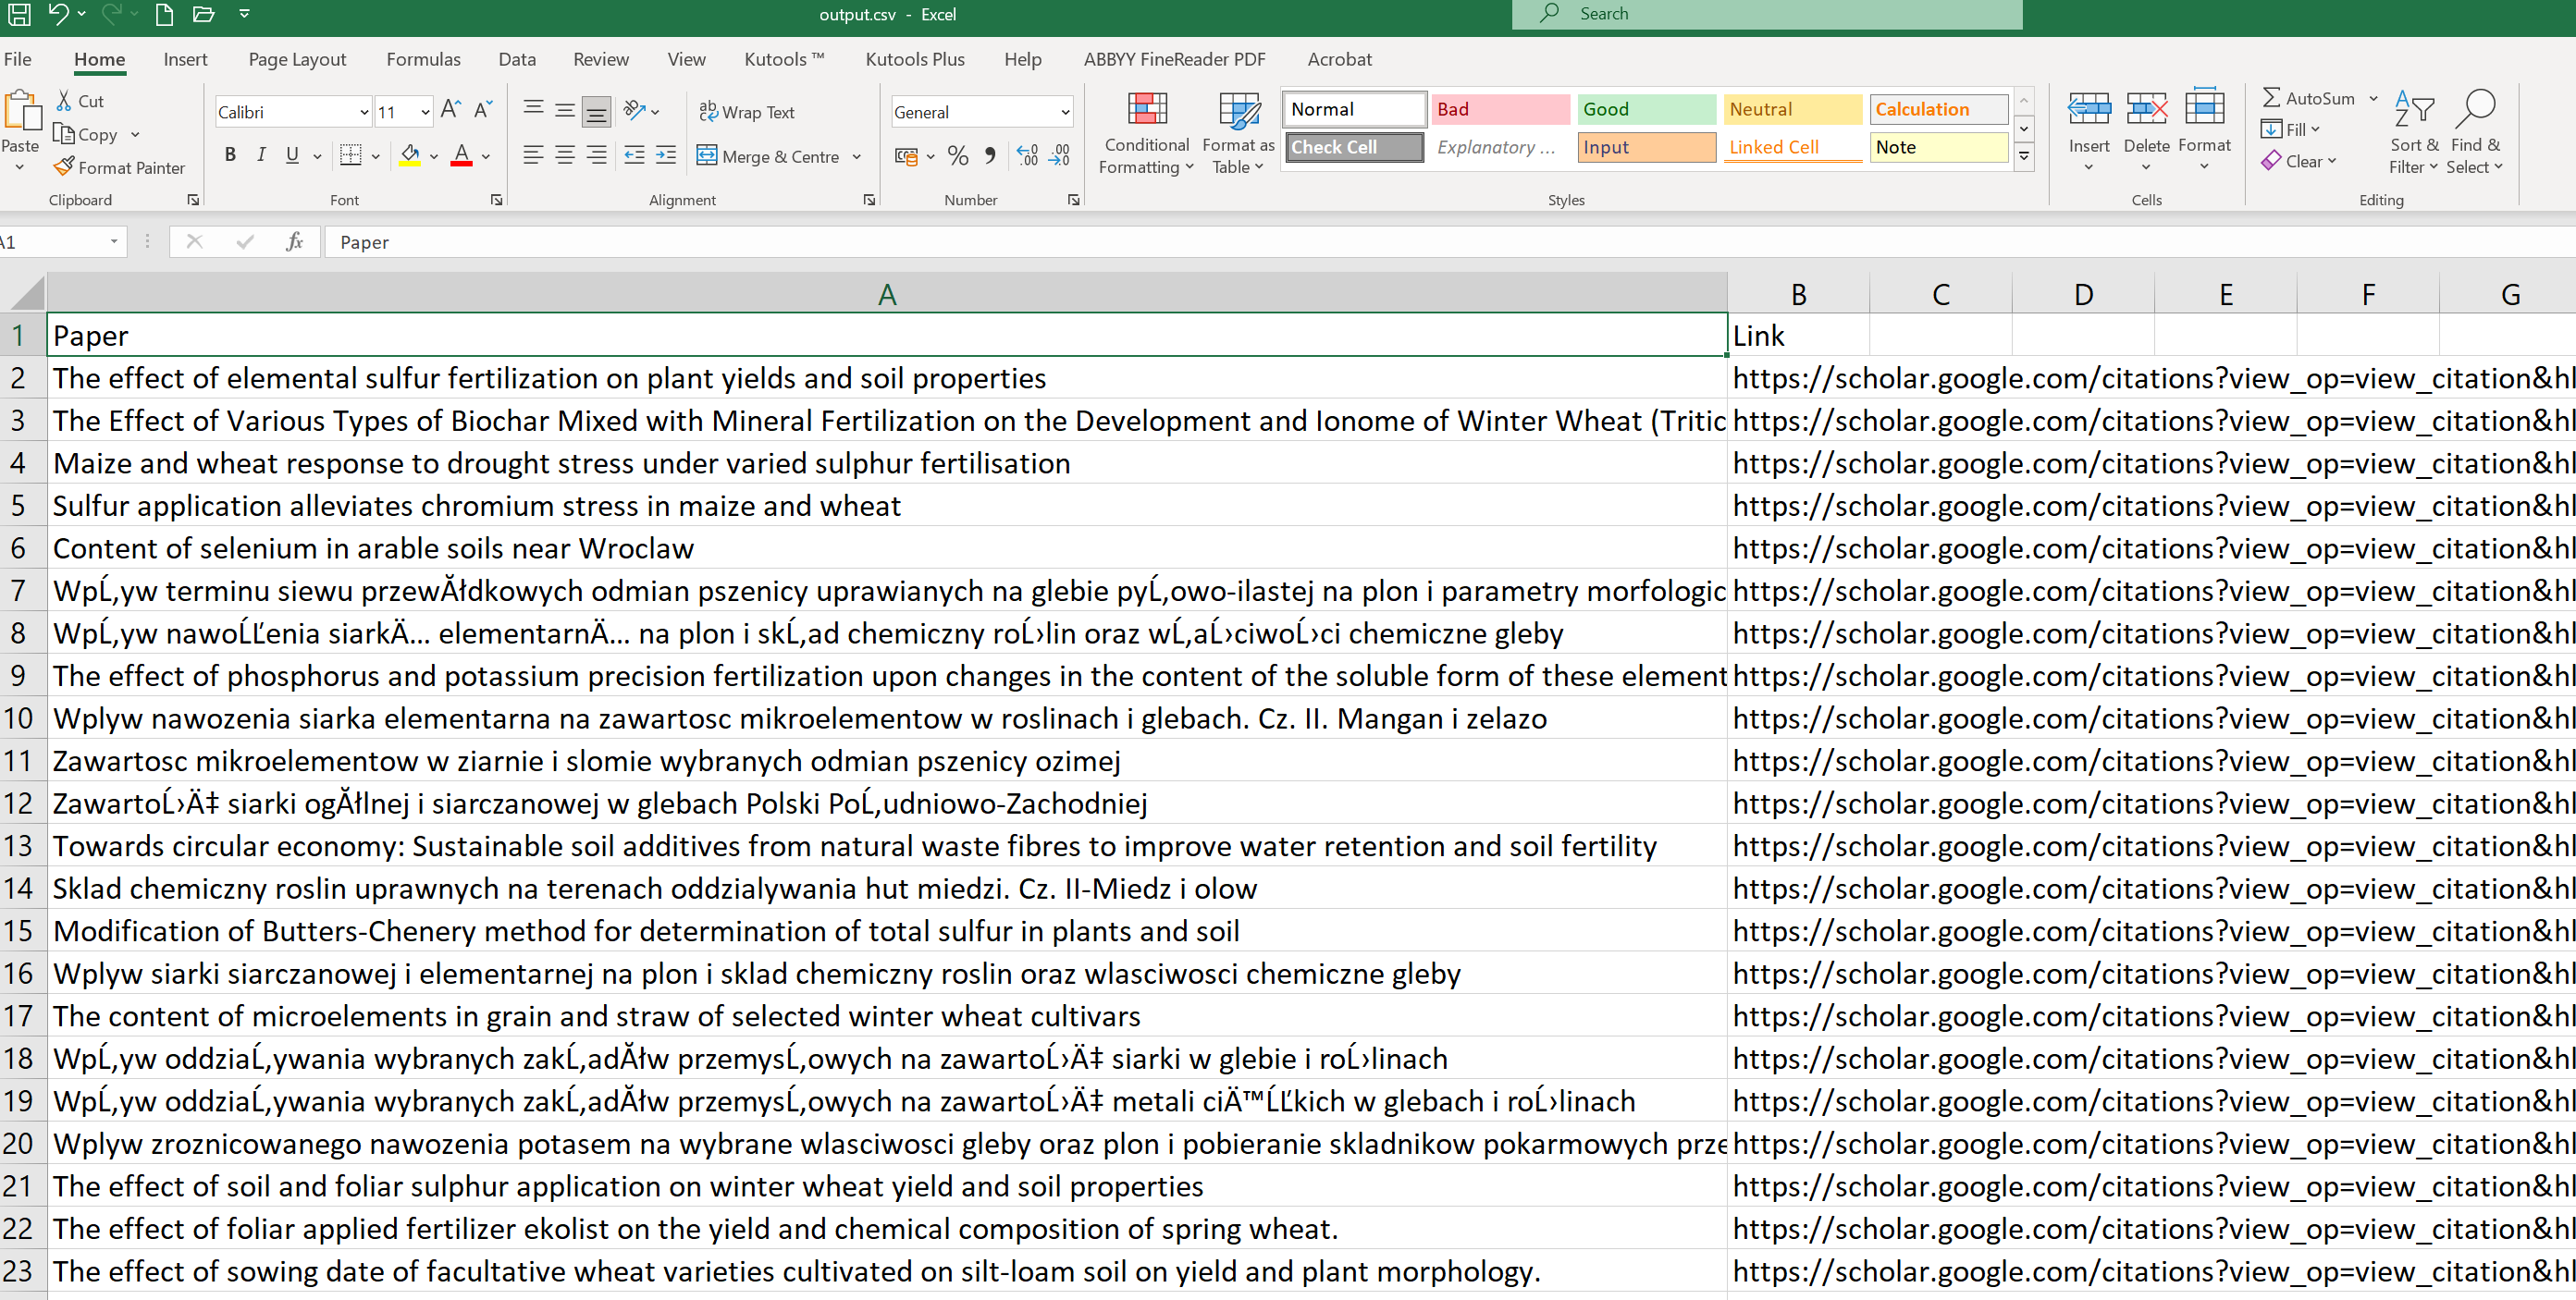
\includegraphics[width=1\textwidth,height=\textheight]{Rysunki/profil_pub_wynik_csv.png}
\caption{Zestawienie publikacji i linków dla wybranego id naukowca
\label{zestawienie_profil_pub}}
\end{figure}

\hypertarget{baza-danych-semantic-scholar-ss}{%
\subsection{Baza danych Semantic Scholar
(SS)}\label{baza-danych-semantic-scholar-ss}}

Przykład wyszukania tytułu publikacji poprzez jej DOI (Digital Object
Identifier), czyli unikalny identyfikator:

\begin{Shaded}
\begin{Highlighting}[]

\CommentTok{\# from semanticscholar import SemanticScholar}
\CommentTok{\# sch = SemanticScholar()}
\CommentTok{\# paper = sch.get\_paper(\textquotesingle{}10.1016/j.jafr.2024.101013\textquotesingle{})}
\CommentTok{\# paper.title}
\end{Highlighting}
\end{Shaded}

Przykład wyszukania autora publikacji poprzez jego numer identyfikujący:

Wyszukanie autora publikacji poprzez jego dane Imię i Nazwisko:

\begin{Shaded}
\begin{Highlighting}[]

\CommentTok{\# from semanticscholar import SemanticScholar}
\CommentTok{\# sch = SemanticScholar()}
\CommentTok{\# results = sch.search\_author(\textquotesingle{}Grzegorz Kulczycki\textquotesingle{})}
\CommentTok{\# print(f\textquotesingle{}\{results.total\} results.\textquotesingle{}, f\textquotesingle{}First occurrence: \{results[0].name\}.\textquotesingle{})}
\end{Highlighting}
\end{Shaded}

\begin{Shaded}
\begin{Highlighting}[]
\CommentTok{\# library(reticulate)}
\CommentTok{\# }
\CommentTok{\# \# Import and run a Python file}
\CommentTok{\# py\_run\_file("Skrypty/test\_skryptu.py")}
\end{Highlighting}
\end{Shaded}

\FloatBarrier
\newpage
\fancyhead[C]{Wnioski}

\hypertarget{wnioski}{%
\section{Wnioski}\label{wnioski}}

\textbf{Na podstawie przeprowadzonych badań wyciągnięto następujące
wnioski:}

\begin{enumerate}
\def\labelenumi{\arabic{enumi}.}
\item
  Środowisko pracy programu R z jego graficznym interfejsem RStudio oraz
  biblioteką R Markdown umożliwia przeprowadzenie tworzenia publikacji
  naukowych w pełni powtarzalnych (rys. \ref{reproducibility_court}).
\item
  R Markdown tworzy dynamiczne dokumenty poprzez możliwość zastosowania
  zagnieżdżonych kodów języków programowania.
\item
  Zastosowanie powtarzalnych metod publikowania pozwala na
  zautomatyzowanie tego procesu przyczyniając się do zwiększenia
  efektywności pracy naukowej.
\item
  Konwersja wyników pracy do różnych formatów stanowi istotną zaletę
  korzystania z tych narzędzi pracy w porównaniu do tradycyjnych metod
  korzystania z popularnych edytorów tekstu.
\item
  Zaletą korzystania z odtwarzalnych metod jest możliwość skupienia się
  na pisaniu pracy bez konieczności zajmowania się problemami edycyjnymi
  przy tworzeniu dokumentu.
\item
  Wymagany początkowy duży nakład pracy w opanowanie środowiska pracy R,
  możne wpływać zniechęcająco na potencjalnych użytkowników tego
  oprogramowania, ale w dłuższej perspektywie zdecydowanie zwiększa
  efektywność pracy przy tworzeniu publikacji naukowych.
\end{enumerate}

\begin{figure}
\centering

\includegraphics[width=0.5\textwidth,height=\textheight]{Rysunki/reproducibility_court.png}
\caption{Potwierdzenie powtarzalności dokumentu (rysunek wykonała
\href{https://github.com/allisonhorst/stats-illustrations/}{Allison
Horst}) \label{reproducibility_court}}
\end{figure}

\FloatBarrier
\newpage
\fancyhead[C]{Literatura}

\hypertarget{literatura}{%
\section{Literatura}\label{literatura}}

\hypertarget{refs}{}
\begin{CSLReferences}{1}{0}
\leavevmode\vadjust pre{\hypertarget{ref-apanowicz2005}{}}%
Apanowicz, J. 2005. Metodologiczne uwarunkowania pracy naukowej. Prace
doktorskie. Prace habilitacyjne. Difin, Warszawa.

\leavevmode\vadjust pre{\hypertarget{ref-chigbu2023}{}}%
Chigbu, U.E., S.O. Atiku, i C.C. Du Plessis. 2023. The Science of
Literature Reviews: Searching, Identifying, Selecting, and Synthesising.
Publications 11(11): 2. doi:
\href{https://doi.org/10.3390/publications11010002}{10.3390/publications11010002}.

\leavevmode\vadjust pre{\hypertarget{ref-comarch2023}{}}%
Comarch. 2023. Ranking najpopularniejszych języków programowania według
TIOBE Index.
\url{https://kariera.comarch.pl/blog/python-na-czele-julia-pierwszy-raz-w-czolowej-dwudziestce-ranking-najpopularniejszych-jezykow-programowania-wedlug-tiobe-index/}.

\leavevmode\vadjust pre{\hypertarget{ref-cooper1986}{}}%
Cooper, H.M. 1986. The integrative research review: a systematic
approach. 2. print. Sage.

\leavevmode\vadjust pre{\hypertarget{ref-curcic2023}{}}%
Curcic, D. 2023. Number of academic papers published per year.
WordsRated.

\leavevmode\vadjust pre{\hypertarget{ref-dz.u.2019}{}}%
Dz. U. 2019. Rozporz{ą}dzenie Ministra Nauki i Szkolnictwa Wy{ż}szego z
dnia 22 lutego 2019 r. w sprawie ewaluacji jako{ś}ci dzia{ł}alno{ś}ci
naukowej Poz. 392.

\leavevmode\vadjust pre{\hypertarget{ref-guxf3recki2011}{}}%
Górecki, T. 2011. Podstawy statystyki z przyk{ł}adami w R. Wydawnictwo
BTC, Legionowo.

\leavevmode\vadjust pre{\hypertarget{ref-kinney2023}{}}%
Kinney, R., C. Anastasiades, R. Authur, I. Beltagy, J. Bragg, i in.
2023. The Semantic Scholar Open Data Platform. doi:
\href{https://doi.org/10.48550/ARXIV.2301.10140}{10.48550/ARXIV.2301.10140}.

\leavevmode\vadjust pre{\hypertarget{ref-pbn2020}{}}%
PBN. 2020. Słownik pojęć Polska Bibliografia Naukowa. Polska
Bibliografia Naukowa.
\url{https://pbn.nauka.gov.pl/centrum-pomocy/baza-wiedzy/slowniczek-pojec/}.

\leavevmode\vadjust pre{\hypertarget{ref-pwn2023}{}}%
PWN. 2023. PWN Nauka.

\leavevmode\vadjust pre{\hypertarget{ref-strus2017}{}}%
Struś, A. 2017. R {Markdown} Narzędzie Do Tworzenia Dynamicznych
Dokumentów i Zestawień.

\leavevmode\vadjust pre{\hypertarget{ref-tranfield2003}{}}%
Tranfield, D., D. Denyer, i P. Smart. 2003. Towards a Methodology for
Developing Evidence-Informed Management Knowledge by Means of Systematic
Review. British Journal of Management 14(3): 207--222. doi:
\href{https://doi.org/10.1111/1467-8551.00375}{10.1111/1467-8551.00375}.

\leavevmode\vadjust pre{\hypertarget{ref-wickham2018}{}}%
Wickham, H., i G. Grolemund. 2018. J{ę}zyk R. Kompletny zestaw
narz{ę}dzi dla analityków danych. Helion, Gliwice.

\leavevmode\vadjust pre{\hypertarget{ref-ziemkiewicz2013}{}}%
Ziemkiewicz, B., i J. Karłowska-Pik. 2013. LATEX dla matematyków.
Wydawnictwo Naukowe UMK Toru{ń}.

\end{CSLReferences}

\FloatBarrier
\newpage
\fancyhead[C]{Spis rysunków}
\listoffigures
\addcontentsline{toc}{section}{Spis rysunków}

\end{document}
